% Options for packages loaded elsewhere
\PassOptionsToPackage{unicode}{hyperref}
\PassOptionsToPackage{hyphens}{url}
%
\documentclass[
]{book}
\usepackage{amsmath,amssymb}
\usepackage{iftex}
\ifPDFTeX
  \usepackage[T1]{fontenc}
  \usepackage[utf8]{inputenc}
  \usepackage{textcomp} % provide euro and other symbols
\else % if luatex or xetex
  \usepackage{unicode-math} % this also loads fontspec
  \defaultfontfeatures{Scale=MatchLowercase}
  \defaultfontfeatures[\rmfamily]{Ligatures=TeX,Scale=1}
\fi
\usepackage{lmodern}
\ifPDFTeX\else
  % xetex/luatex font selection
\fi
% Use upquote if available, for straight quotes in verbatim environments
\IfFileExists{upquote.sty}{\usepackage{upquote}}{}
\IfFileExists{microtype.sty}{% use microtype if available
  \usepackage[]{microtype}
  \UseMicrotypeSet[protrusion]{basicmath} % disable protrusion for tt fonts
}{}
\makeatletter
\@ifundefined{KOMAClassName}{% if non-KOMA class
  \IfFileExists{parskip.sty}{%
    \usepackage{parskip}
  }{% else
    \setlength{\parindent}{0pt}
    \setlength{\parskip}{6pt plus 2pt minus 1pt}}
}{% if KOMA class
  \KOMAoptions{parskip=half}}
\makeatother
\usepackage{xcolor}
\usepackage{color}
\usepackage{fancyvrb}
\newcommand{\VerbBar}{|}
\newcommand{\VERB}{\Verb[commandchars=\\\{\}]}
\DefineVerbatimEnvironment{Highlighting}{Verbatim}{commandchars=\\\{\}}
% Add ',fontsize=\small' for more characters per line
\usepackage{framed}
\definecolor{shadecolor}{RGB}{248,248,248}
\newenvironment{Shaded}{\begin{snugshade}}{\end{snugshade}}
\newcommand{\AlertTok}[1]{\textcolor[rgb]{0.94,0.16,0.16}{#1}}
\newcommand{\AnnotationTok}[1]{\textcolor[rgb]{0.56,0.35,0.01}{\textbf{\textit{#1}}}}
\newcommand{\AttributeTok}[1]{\textcolor[rgb]{0.13,0.29,0.53}{#1}}
\newcommand{\BaseNTok}[1]{\textcolor[rgb]{0.00,0.00,0.81}{#1}}
\newcommand{\BuiltInTok}[1]{#1}
\newcommand{\CharTok}[1]{\textcolor[rgb]{0.31,0.60,0.02}{#1}}
\newcommand{\CommentTok}[1]{\textcolor[rgb]{0.56,0.35,0.01}{\textit{#1}}}
\newcommand{\CommentVarTok}[1]{\textcolor[rgb]{0.56,0.35,0.01}{\textbf{\textit{#1}}}}
\newcommand{\ConstantTok}[1]{\textcolor[rgb]{0.56,0.35,0.01}{#1}}
\newcommand{\ControlFlowTok}[1]{\textcolor[rgb]{0.13,0.29,0.53}{\textbf{#1}}}
\newcommand{\DataTypeTok}[1]{\textcolor[rgb]{0.13,0.29,0.53}{#1}}
\newcommand{\DecValTok}[1]{\textcolor[rgb]{0.00,0.00,0.81}{#1}}
\newcommand{\DocumentationTok}[1]{\textcolor[rgb]{0.56,0.35,0.01}{\textbf{\textit{#1}}}}
\newcommand{\ErrorTok}[1]{\textcolor[rgb]{0.64,0.00,0.00}{\textbf{#1}}}
\newcommand{\ExtensionTok}[1]{#1}
\newcommand{\FloatTok}[1]{\textcolor[rgb]{0.00,0.00,0.81}{#1}}
\newcommand{\FunctionTok}[1]{\textcolor[rgb]{0.13,0.29,0.53}{\textbf{#1}}}
\newcommand{\ImportTok}[1]{#1}
\newcommand{\InformationTok}[1]{\textcolor[rgb]{0.56,0.35,0.01}{\textbf{\textit{#1}}}}
\newcommand{\KeywordTok}[1]{\textcolor[rgb]{0.13,0.29,0.53}{\textbf{#1}}}
\newcommand{\NormalTok}[1]{#1}
\newcommand{\OperatorTok}[1]{\textcolor[rgb]{0.81,0.36,0.00}{\textbf{#1}}}
\newcommand{\OtherTok}[1]{\textcolor[rgb]{0.56,0.35,0.01}{#1}}
\newcommand{\PreprocessorTok}[1]{\textcolor[rgb]{0.56,0.35,0.01}{\textit{#1}}}
\newcommand{\RegionMarkerTok}[1]{#1}
\newcommand{\SpecialCharTok}[1]{\textcolor[rgb]{0.81,0.36,0.00}{\textbf{#1}}}
\newcommand{\SpecialStringTok}[1]{\textcolor[rgb]{0.31,0.60,0.02}{#1}}
\newcommand{\StringTok}[1]{\textcolor[rgb]{0.31,0.60,0.02}{#1}}
\newcommand{\VariableTok}[1]{\textcolor[rgb]{0.00,0.00,0.00}{#1}}
\newcommand{\VerbatimStringTok}[1]{\textcolor[rgb]{0.31,0.60,0.02}{#1}}
\newcommand{\WarningTok}[1]{\textcolor[rgb]{0.56,0.35,0.01}{\textbf{\textit{#1}}}}
\usepackage{longtable,booktabs,array}
\usepackage{calc} % for calculating minipage widths
% Correct order of tables after \paragraph or \subparagraph
\usepackage{etoolbox}
\makeatletter
\patchcmd\longtable{\par}{\if@noskipsec\mbox{}\fi\par}{}{}
\makeatother
% Allow footnotes in longtable head/foot
\IfFileExists{footnotehyper.sty}{\usepackage{footnotehyper}}{\usepackage{footnote}}
\makesavenoteenv{longtable}
\usepackage{graphicx}
\makeatletter
\def\maxwidth{\ifdim\Gin@nat@width>\linewidth\linewidth\else\Gin@nat@width\fi}
\def\maxheight{\ifdim\Gin@nat@height>\textheight\textheight\else\Gin@nat@height\fi}
\makeatother
% Scale images if necessary, so that they will not overflow the page
% margins by default, and it is still possible to overwrite the defaults
% using explicit options in \includegraphics[width, height, ...]{}
\setkeys{Gin}{width=\maxwidth,height=\maxheight,keepaspectratio}
% Set default figure placement to htbp
\makeatletter
\def\fps@figure{htbp}
\makeatother
\setlength{\emergencystretch}{3em} % prevent overfull lines
\providecommand{\tightlist}{%
  \setlength{\itemsep}{0pt}\setlength{\parskip}{0pt}}
\setcounter{secnumdepth}{5}
\usepackage{booktabs}
\usepackage{color}
\usepackage{framed}
\setlength{\fboxsep}{.8em}

% These colours were manually entered, they shouldn't matter unless you want pdf output

\newenvironment{redbox}{
  \definecolor{shadecolor}{RGB}{243, 154, 157}
  \color{white}
  \begin{shaded}}
 {\end{shaded}}

\newenvironment{bluebox}{
  \definecolor{shadecolor}{RGB}{172, 210, 237}
  \color{white}
  \begin{shaded}}
 {\end{shaded}}

\newenvironment{greenbox}{
  \definecolor{shadecolor}{RGB}{141, 181, 128}
  \color{white}
  \begin{shaded}}
 {\end{shaded}}
\ifLuaTeX
  \usepackage{selnolig}  % disable illegal ligatures
\fi
\usepackage[]{natbib}
\bibliographystyle{plainnat}
\usepackage{bookmark}
\IfFileExists{xurl.sty}{\usepackage{xurl}}{} % add URL line breaks if available
\urlstyle{same}
\hypersetup{
  pdftitle={CBW's Bookdown Template Documentation},
  hidelinks,
  pdfcreator={LaTeX via pandoc}}

\title{CBW's Bookdown Template Documentation}
\author{}
\date{\vspace{-2.5em}Last Updated: 2024-12-15}

\usepackage{amsthm}
\newtheorem{theorem}{Theorem}[chapter]
\newtheorem{lemma}{Lemma}[chapter]
\newtheorem{corollary}{Corollary}[chapter]
\newtheorem{proposition}{Proposition}[chapter]
\newtheorem{conjecture}{Conjecture}[chapter]
\theoremstyle{definition}
\newtheorem{definition}{Definition}[chapter]
\theoremstyle{definition}
\newtheorem{example}{Example}[chapter]
\theoremstyle{definition}
\newtheorem{exercise}{Exercise}[chapter]
\theoremstyle{definition}
\newtheorem{hypothesis}{Hypothesis}[chapter]
\theoremstyle{remark}
\newtheorem*{remark}{Remark}
\newtheorem*{solution}{Solution}
\begin{document}
\maketitle

{
\setcounter{tocdepth}{1}
\tableofcontents
}
\chapter{CBW's Bookdown Documentation}\label{cbws-bookdown-documentation}

Welcome to CBW's documentation for creating a workshop website using Bookdown. Bookdown is an R package that is used to build books, and in our case, the websites hosting CBW's workshops!

You only need to know markdown and whatever coding language you will be using to learn bookdown!

Note, this is the documentation to create a workshop using \emph{bookdown}. If \textbf{Jupyter Book} suits you better, see \href{https://cbw-dev.github.io/jupyterbook-docs/}{here}.

If you don't know which one to use, click \href{}{here} to learn more!

\chapter{Getting Started}\label{get-started}

Bookdown is an open-source R package that helps write books and articles. We will be building our bookdown-based workshop websites using this, specifically the gitbook template. (This is just the name of the specific template style, you will be working in a workshop template that CBW has prepared for you!)

If you're ready to start making a workshop website in bookdown, let's setup your device (PC, laptop)!

First, let's explain installations.

\section{Installation}\label{installation}

Since bookdown is an R package, you will need R. Plus, our ideal IDE (integrated development environment i.e.~the platform we will be working in) is RStudio.

\begin{enumerate}
\def\labelenumi{\arabic{enumi}.}
\item
  \textbf{Download and install R} here. (You need R 3.6.0+ installed for RStudio.) Follow the instructions for your operating system (Linux/macOS/Windows).

  \begin{quote}
  Check: You can check if windows was installed properly on \emph{macOS} by running the command \texttt{R} in terminal. On \emph{windows}, --must test--.
  \end{quote}

  \begin{quote}
  Note: We will not be using the R console, instead, we will be using RStudio!
  \end{quote}
\item
  \textbf{Download and install RStudio} here. Scroll down to find downloads for non-macOS.

  \begin{quote}
  Note: While installing, you may be asked whether to install the 32-bit or 62-bit RStudio version. Download the version that matches your PC.
  \end{quote}
\item
  \textbf{Install Git, if you don't already have it.} Git is a tool that will help us with version control when editing your workshop. Linux and macOS computers tend to have Git installed. Windows computers must install Git. However, make sure to double check if you already have Git, so that you don't have to install it again! Check if you have Git by running this command in terminal/command prompt:

\begin{Shaded}
\begin{Highlighting}[]
\FunctionTok{git} \AttributeTok{{-}{-}version}
\end{Highlighting}
\end{Shaded}

\begin{verbatim}
## git version 2.39.5 (Apple Git-154)
\end{verbatim}

  If your output looks like ``git version X.X.X \ldots{}'', you already have git! Move onto step 4!

  However, if your output says ``Git is not recognized'' or a similar statement (such as the one provided below), you do not have Git, so you must install it as well.

\begin{verbatim}
'git' is not recognized as an internal or external command,
operable program or batch file.
\end{verbatim}

  \textbf{Installing Git on macOS}

  \begin{itemize}
  \tightlist
  \item
    When you ran \texttt{git\ -\/-version}, it will have prompted you to install Git. Follow these instructions.
  \end{itemize}

  \textbf{Installing Git on Windows}

  \begin{itemize}
  \tightlist
  \item
    Go to the Git for Windows installer and download Git. Then, install it with all the default settings.
  \end{itemize}

  Click here for instructions on \textbf{installing Git on Linux}.

  \begin{greenbox}

  \begin{center}
  \textbf{Double Check!}

  \end{center}

  Check that your install worked! Re-run ``git -\/-verison'' and check that you get your git version! (On Windows, this may look like ``git version 2.47.1.windows.1'').

  \begin{quote}
  Note: If you installed Git while having a Command Prompt/Windows PowerShell window open, close this window and open a new one to run ``git -\/-version''. This acts as a refresher to Command Prompt/Windows PowerShell.
  \end{quote}

  \end{greenbox}
\item
  \textbf{Install the bookdown R package}: Open RStudio and in the console (in the bottom left window of RStudio) run the following command: \texttt{install.packages("bookdown")}.

  \begin{itemize}
  \item
    \textbf{Download all the packages you will need!} Do this by running the following command:

\begin{Shaded}
\begin{Highlighting}[]
\FunctionTok{install.packages}\NormalTok{(}\FunctionTok{c}\NormalTok{(}\StringTok{"magrittr"}\NormalTok{, }\StringTok{"stringi"}\NormalTok{, }\StringTok{"stringr"}\NormalTok{, }\StringTok{"reticulate"}\NormalTok{, }\StringTok{"tinytex"}\NormalTok{,}\StringTok{"servr"}\NormalTok{))}
\end{Highlighting}
\end{Shaded}

    You may have to approve some downloads. Say ``yes'' and enter your password when necessary. This tells bookdown you are okay with downloading and installing these packages in their default locations.

    Finally, \textbf{run the following command}

\begin{Shaded}
\begin{Highlighting}[]
\NormalTok{tinytex}\SpecialCharTok{::}\FunctionTok{install\_tinytex}\NormalTok{()}
\end{Highlighting}
\end{Shaded}
  \end{itemize}
\end{enumerate}

We're ready to start working with CBW's bookdown workshop template now!

\begin{bluebox}

\begin{center}
\textbf{Go to the next step}

\end{center}

Now that you're done the installations, it's time to go to the next step: \hyperref[rc-workshop-setup]{creating a \textbf{new} workshop}, if you're a RC, or \hyperref[check-deploy]{seeing your deployed website} (skip to step 4), if you're on the workshop team. The order of this documentation is provided in the sidebar on the left. You can also click the arrows below, to go to the previous or subsequent page!

\end{bluebox}

\chapter{\texorpdfstring{\textbf{New Workshop}: Creation {[}RC{]} and Deployment}{New Workshop: Creation {[}RC{]} and Deployment}}\label{new-workshop-create-deploy}

Certain aspects of the setup for workshops will be different depending on your role. Headers ending in ``{[}RC{]}'' are for Regional Coordinators. Headers without ``{[}RC{]}'' are assumed to be relevant to both RC and workshop teams.

\section{Setup the Workshop {[}RC{]}}\label{rc-workshop-setup}

\begin{enumerate}
\def\labelenumi{\arabic{enumi}.}
\item
  First, let's go to the bookdown template.
\item
  Click on the ``Use this template'' green button, which is to the left of the title of the repository ``bookdown-template''. Then, press the dropdown option: ``Create a new repository'', as seen below.

  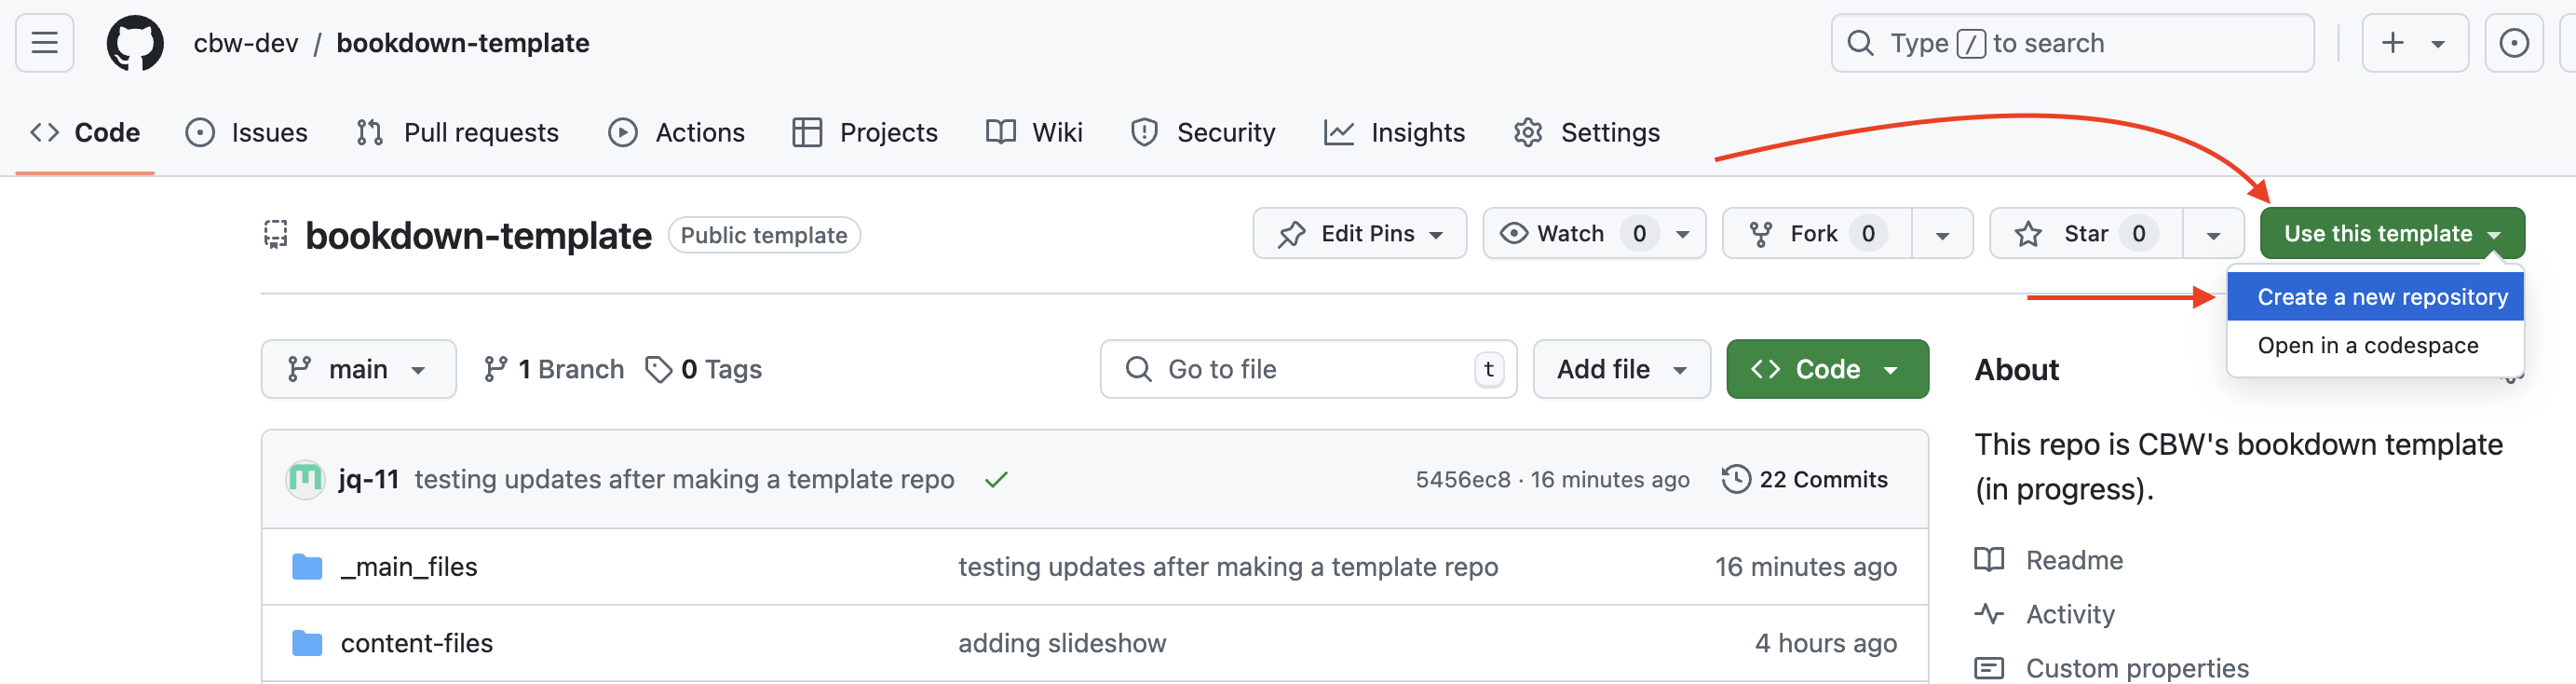
\includegraphics{img/template/make-a-template.png}\\
\item
  You will be brought to a ``Create a new repository'' page. Fill out the blanks as seen below. That is, change the owner to ``bioinformatics.ca'' {[}NOTE FOR TESTING PURPOSES: use cbw-dev{]}, make it public, fill in the repository name and description according to \href{}{CBW Guidelines}. ``Include all branches'' does not need to be selected.

  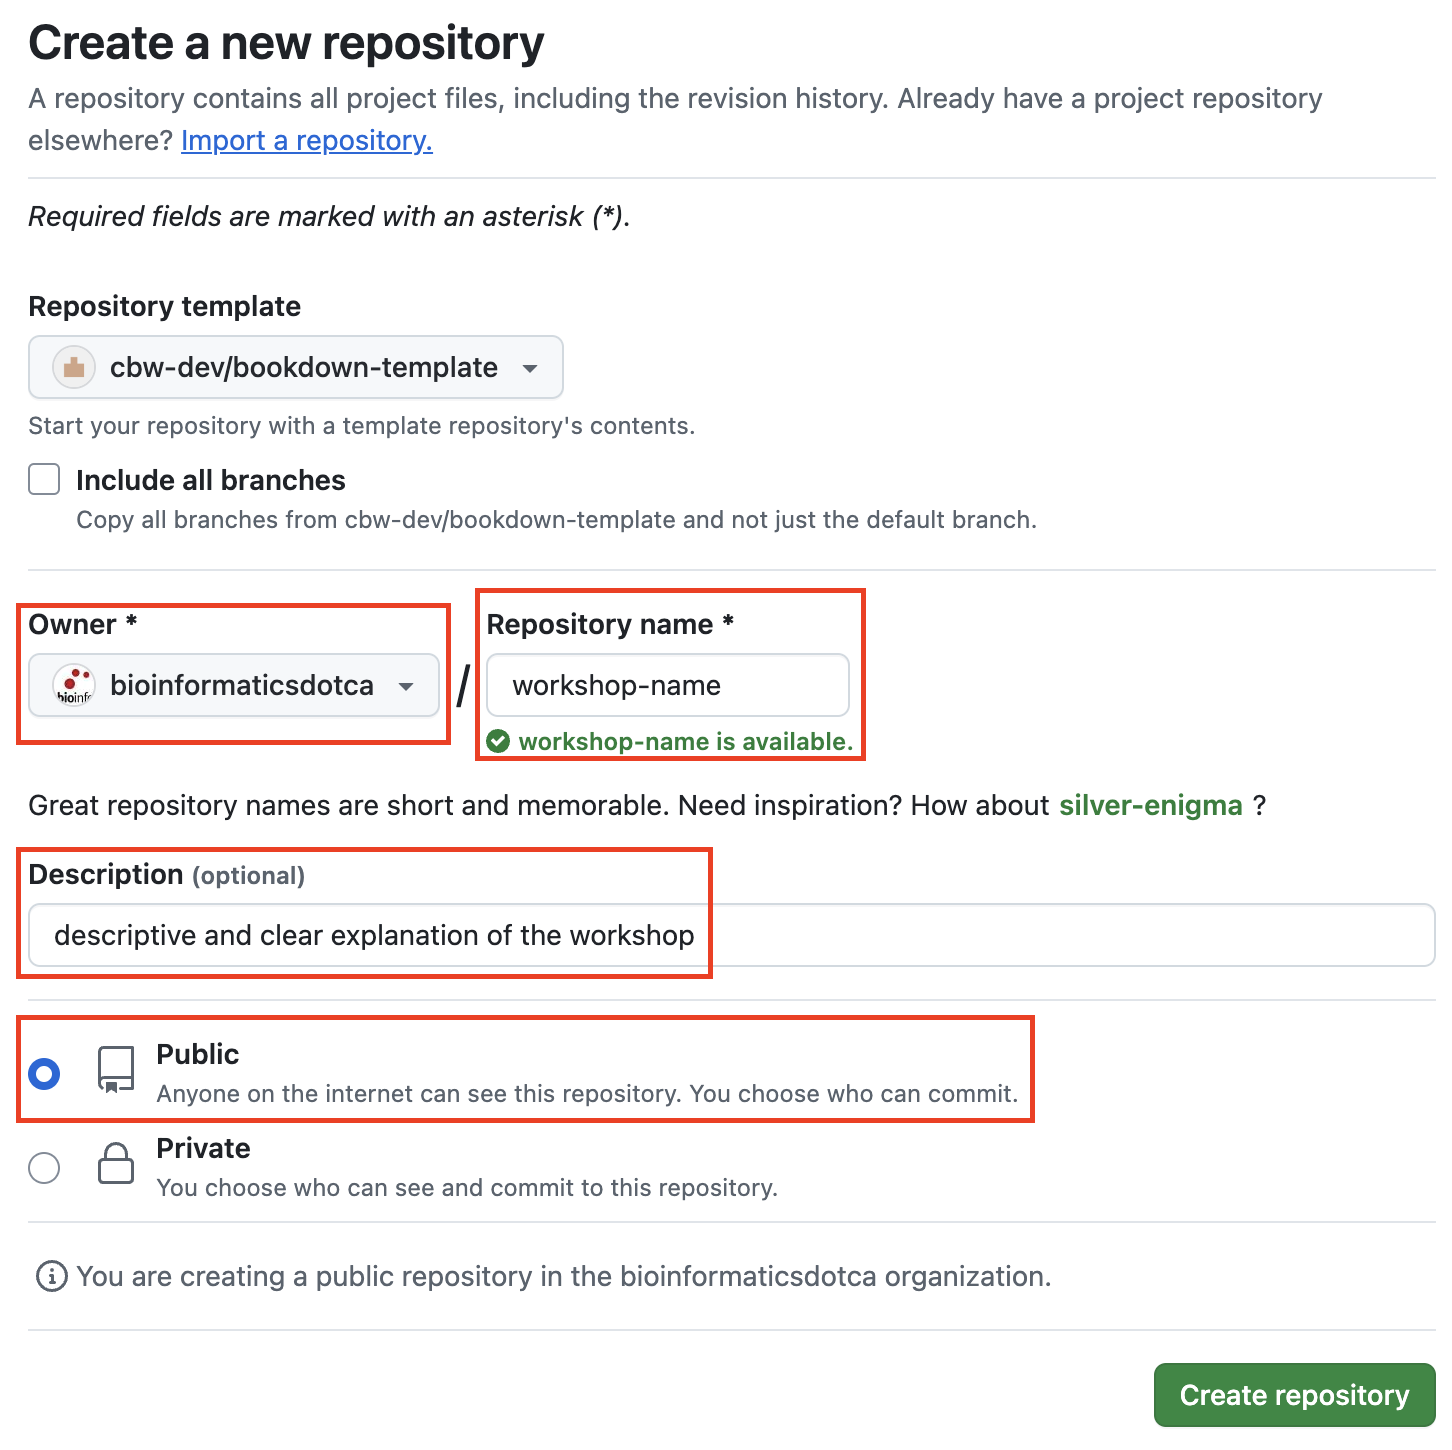
\includegraphics{img/template/make-new-repo.png}\\

  This may take a couple seconds to generate. After it loads, you will be brought to a new repository for the new workshop!

  Now, let's turn this into a website - let's deploy!
\end{enumerate}

\subsection{Workshop Repo VS Workshop Website}\label{workshop-vs-repo}

Now, you have made a repository that holds what GitHub needs to make our website (the basic workshop template). Essentially, the template has already been configured so that the html files that make up our website go into a folder called \texttt{docs}. We need to tell GitHub to look at the \texttt{docs} folder to find our website files and make it available to see online (a.k.a deploy it). This is what we mean when we say CBW uses GitHub pages to deploy our website.

\begin{quote}
Distinction:

GitHub (ex. \url{https://github.com/cbw-dev/bookdown-template}) holds your repo, which has version control for all your files! The deployed website (ex. \url{https://cbw-dev.github.io/bookdown-template/}) has the workshop online.
\end{quote}

\subsection{How to Deploy Your Workshop Website}\label{deploy-website}

\begin{enumerate}
\def\labelenumi{\arabic{enumi}.}
\item
  In the top navigation bar, select settings.
  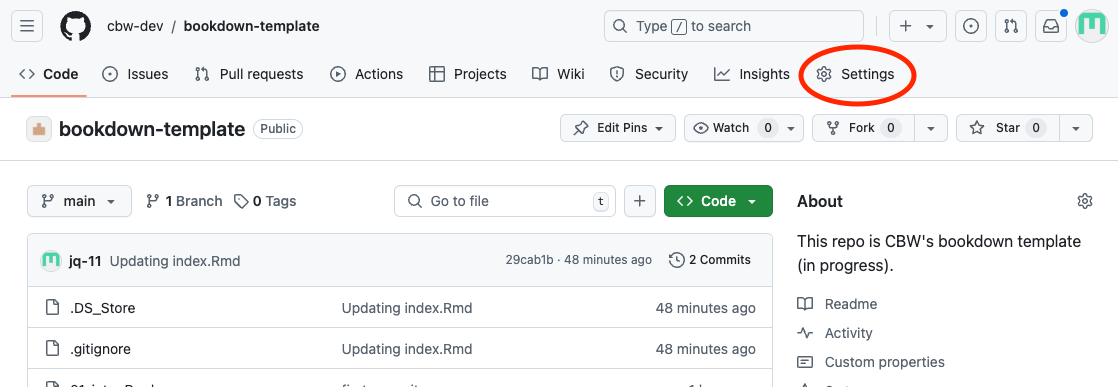
\includegraphics{img/git-instruct/github-settings.png}
\item
  Then, go to the pages sidebar.
  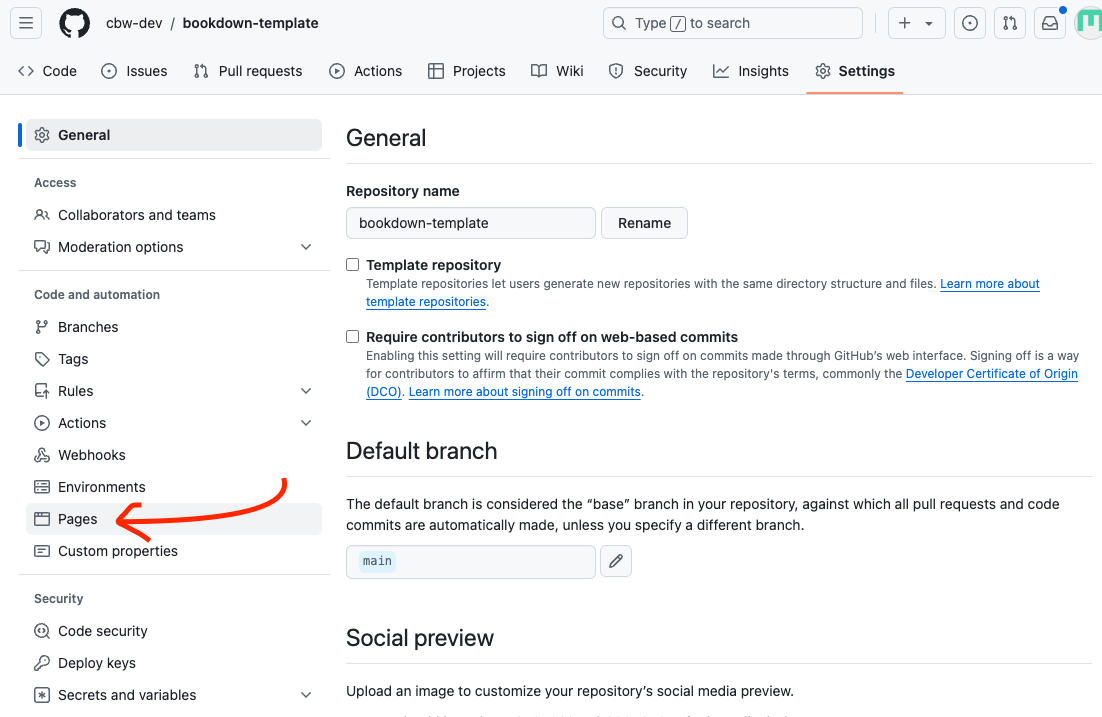
\includegraphics{img/git-instruct/github-select-pages.png}
\item
  ``Deploy from a branch'' is already selected, which is what we want. We must change the branch from ``none'' to ``main''. Select the ``None'' dropdown button and select ``main''.
  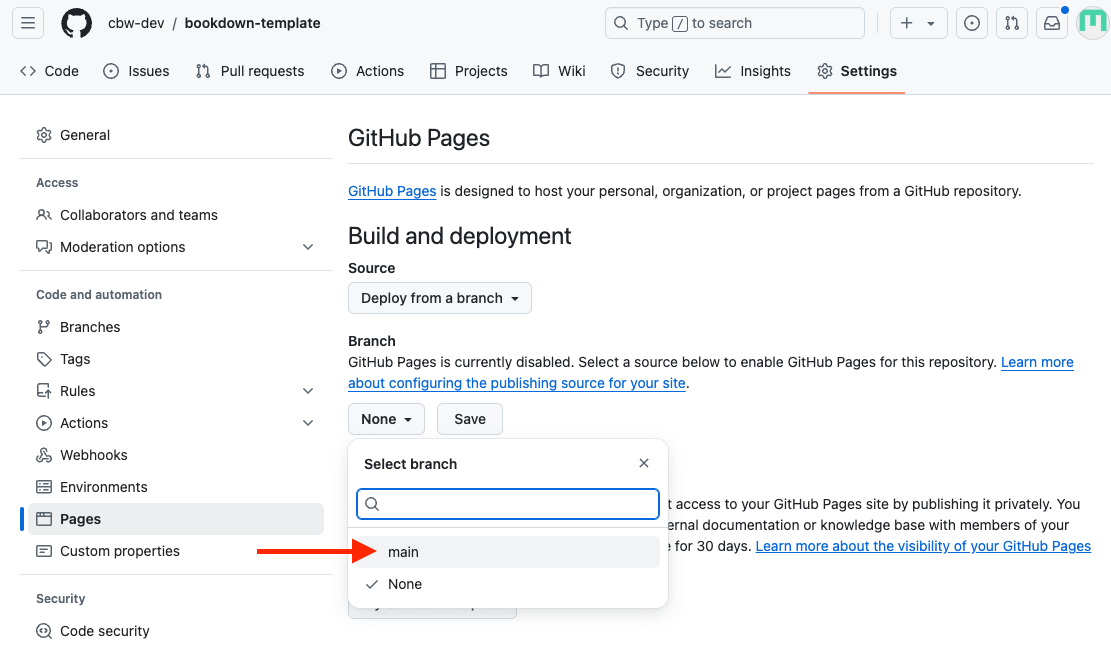
\includegraphics{img/git-instruct/github-deploy-main.png}\\
\item
  Then, change the folder from \texttt{/\ root} to \texttt{/docs}. Then \textbf{press save}.
  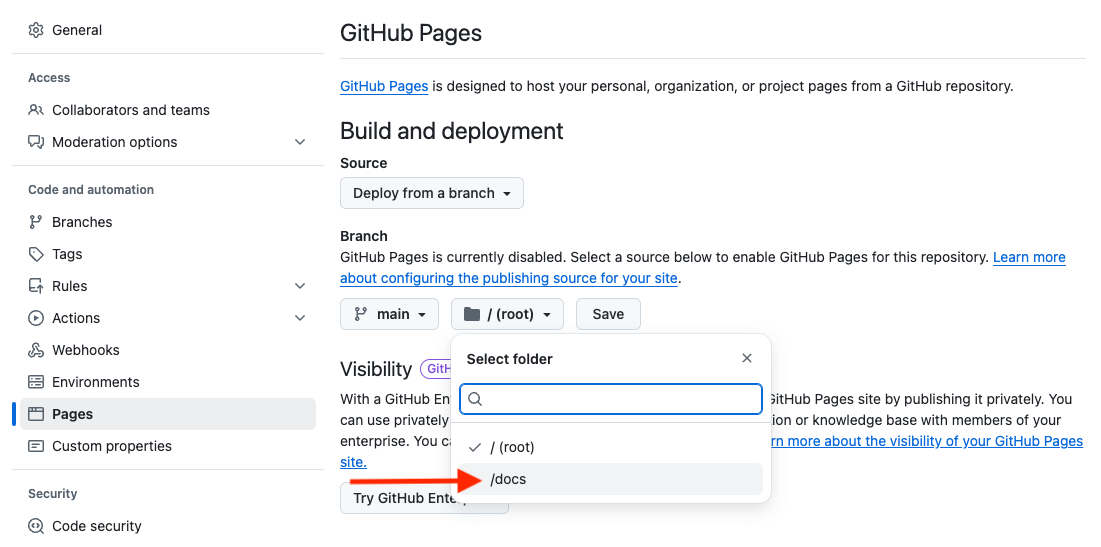
\includegraphics{img/git-instruct/github-deploy-docs.png}\\

  Great! Now we're waiting on the page to build and deploy, which should take less than a minute.
\end{enumerate}

\section{Check Your Deploy and See your Website!}\label{check-deploy}

To see updates, go to the \textbf{Actions} page (found along the top navigation bar. This will help you understand how the deploy is working, and if it succeeded or failed.

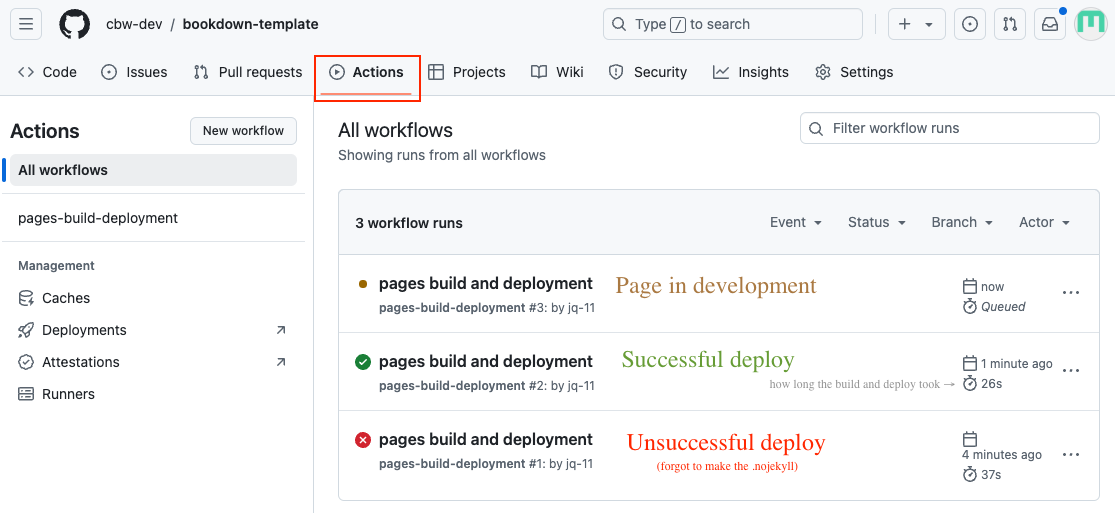
\includegraphics{img/git-instruct/github-pages-actions-explained.png}\\

You can click \textbf{pages build and deployment} for updates.

\begin{figure}
\centering
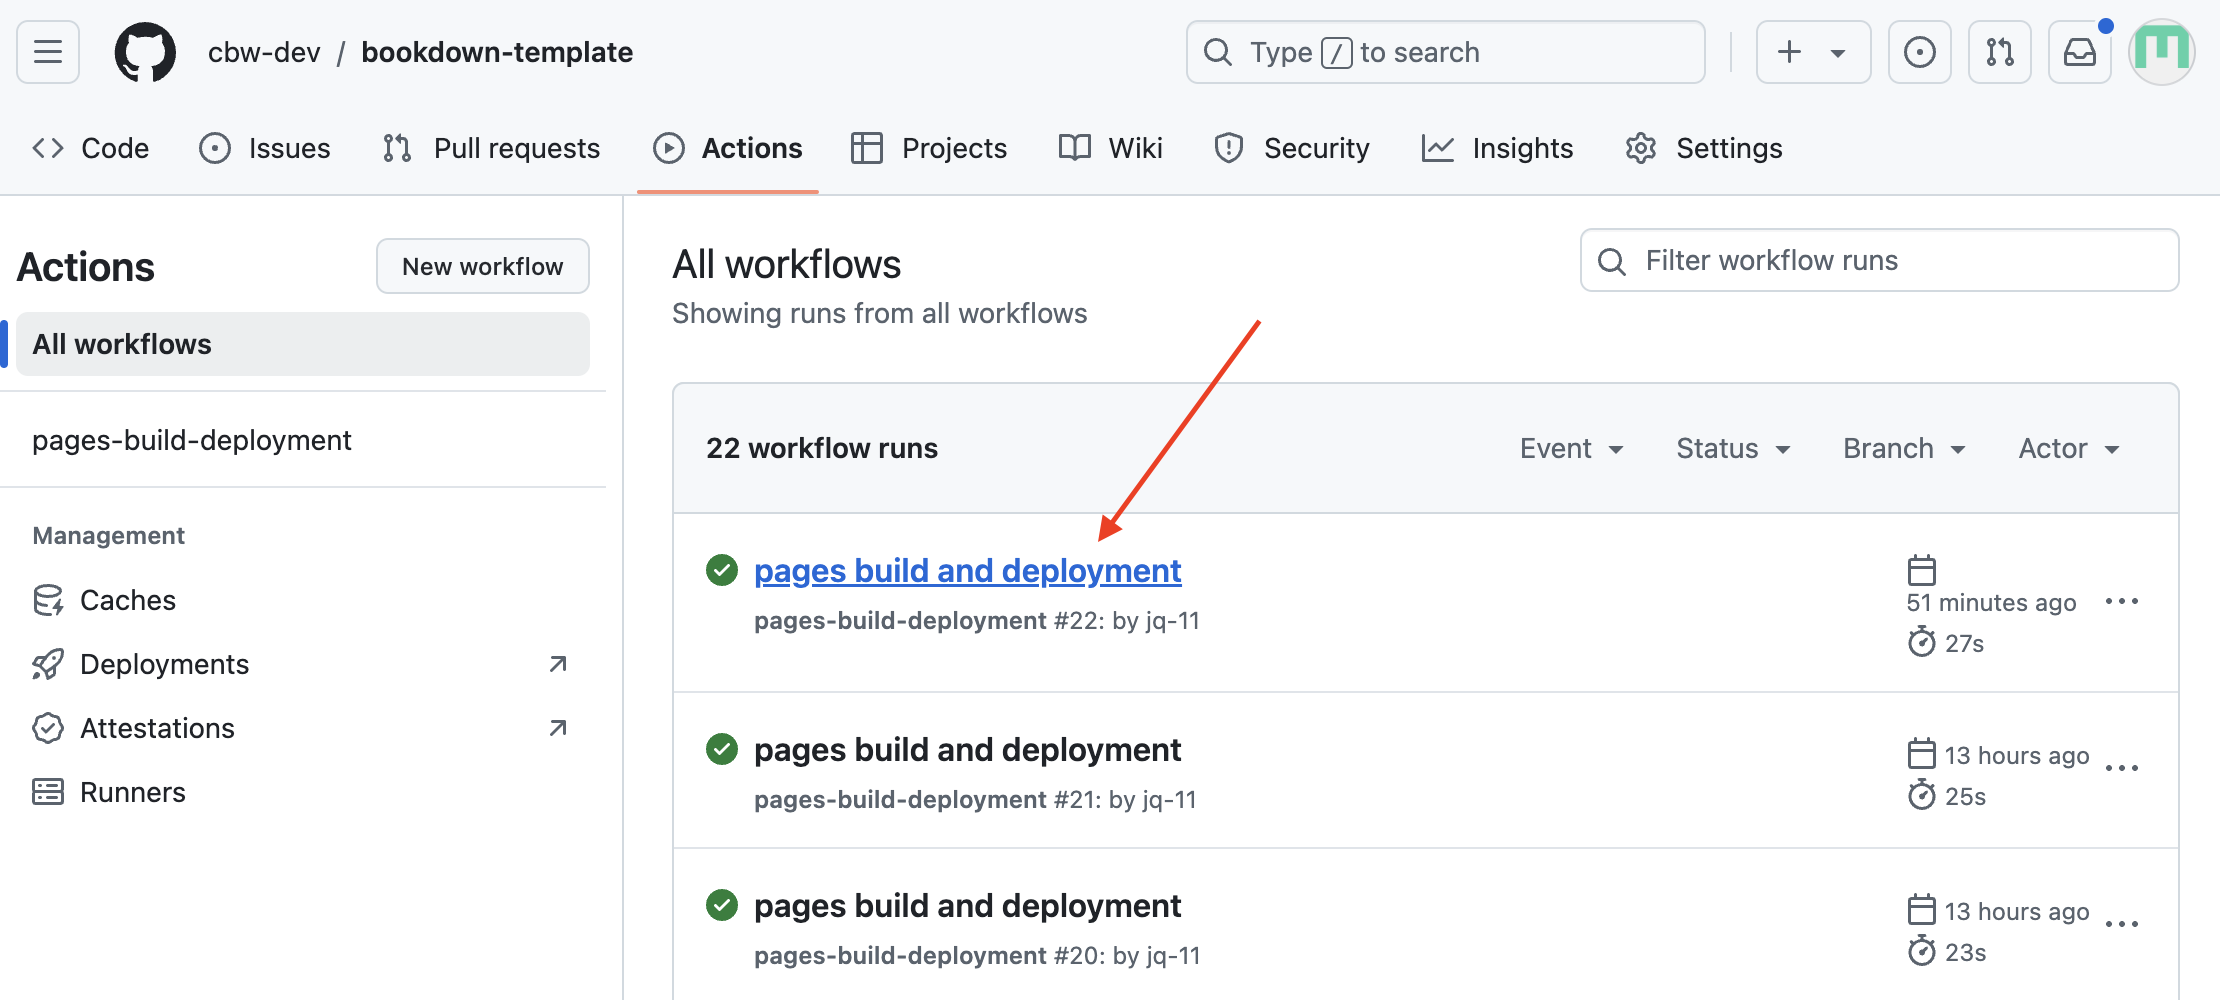
\includegraphics{img/git-instruct/pages-build-and-deployment.png}
\caption{where to click for pages build and deployment information}
\end{figure}

A successful deploy will have a green checkmark next to it. You can inspect the 3 steps: build, report-build-status, deploy. Once it's done deploying, you can find the website at the link provided under ``deploy''!

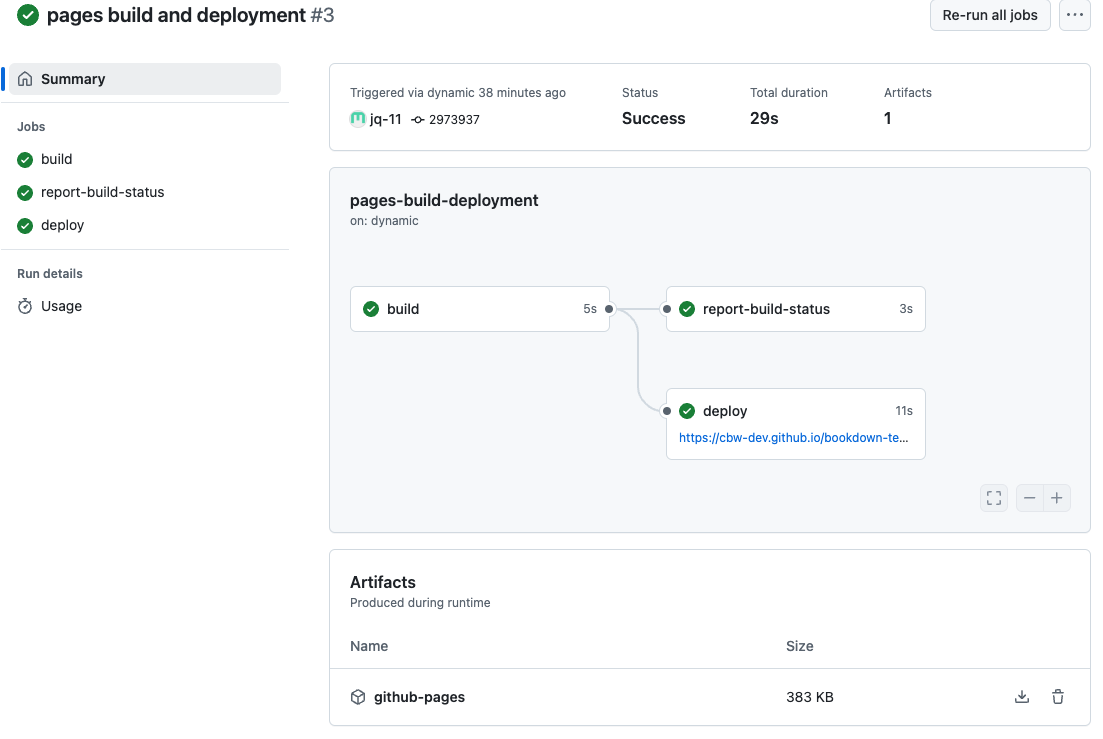
\includegraphics{img/git-instruct/successful-deploy.png}\\

A failed deploy will have a red cross next to it. Clicking through the steps can help you determine what went wrong in the deploy.

\begin{quote}
Warning: A website can build properly, but may not deploy properly! It is a good idea to check after making big changes.
\end{quote}

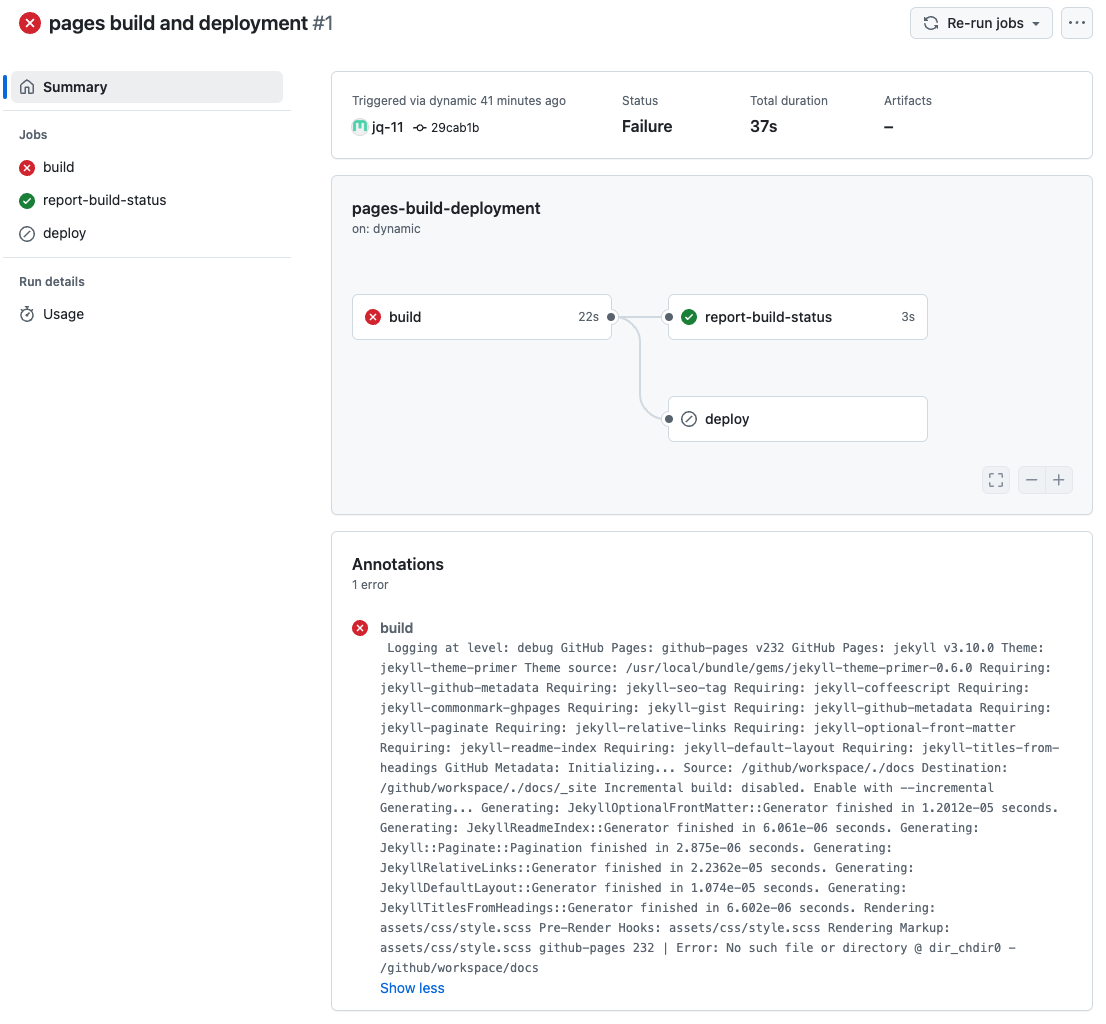
\includegraphics{img/git-instruct/failed-deploy.png}\\

\subsubsection*{A Very Specific Build and Deployment Warning}\label{a-very-specific-build-and-deployment-warning}
\addcontentsline{toc}{subsubsection}{A Very Specific Build and Deployment Warning}

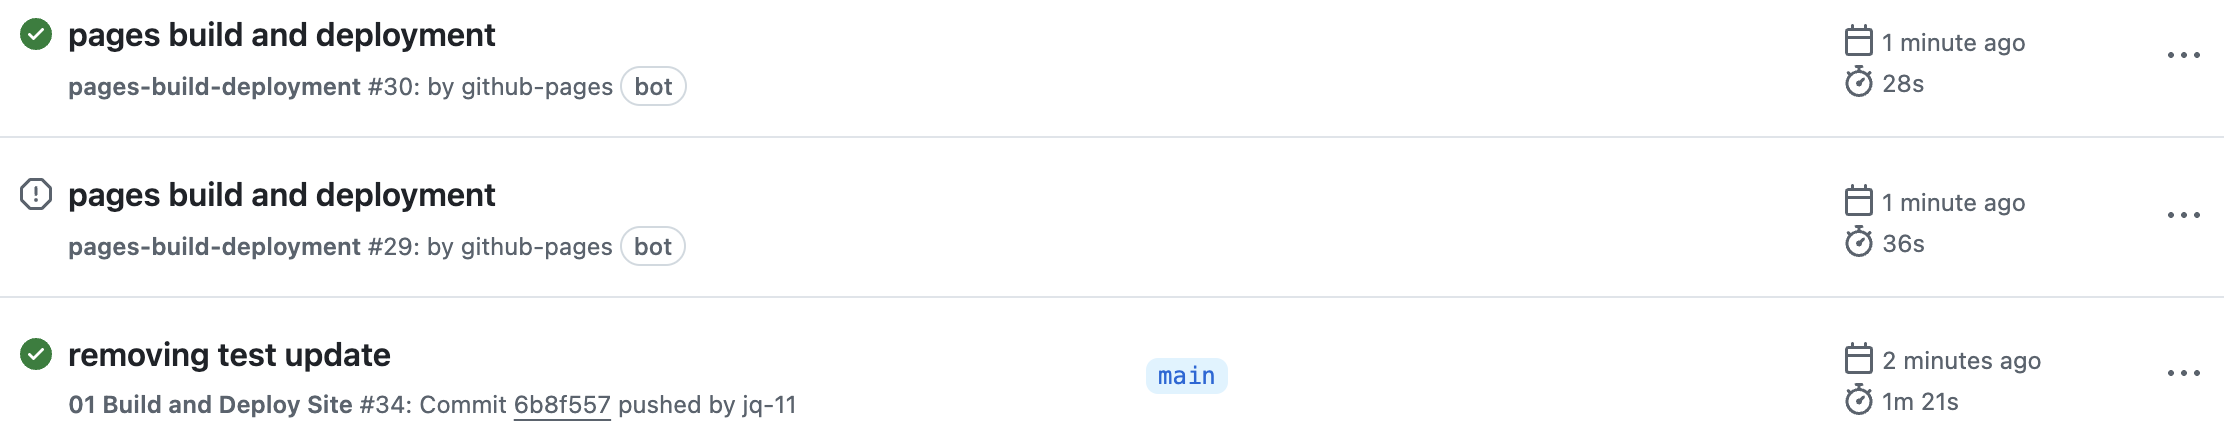
\includegraphics{img/git-instruct/exclamation-point-deploy-warning.png}\\

This is a very specific (and unlikely) warning. It occurs when 1 deploy hasn't finished, but another deploy began. THIS IS NOT A CONCERN. This is a warning message you do not have to worry about!

\section{Setting Up Team Access {[}RC?{]} (Nia will fill this in)}\label{setting-up-team-access-rc-nia-will-fill-this-in}

\chapter{\texorpdfstring{\textbf{Recurring Workshop}: Copying {[}RC{]} and Deployment}{Recurring Workshop: Copying {[}RC{]} and Deployment}}\label{recurring-workshop-copying-rc-and-deployment}

Certain aspects of the setup for workshops will be different depending on your role. Headers ending in ``{[}RC{]}'' are for Regional Coordinators. Headers without ``{[}RC{]}'' are assumed to be relevant to both RC and workshop teams.

\begin{greenbox}

\begin{center}
\textbf{How's this different than the \hyperref[new-workshop-create-deploy]{New Workshop: Creation {[}RC{]} and Deployment} page?}

\end{center}

You should be on this page if CBW already has a version of this workshop as a website, and you mainly wanted to reuse it (maybe with some edits).

\end{greenbox}

\section{Recreate the Workshop}\label{recreate-the-workshop}

We will be creating a copy the existing workshop and workshop website by git forking the repository that hosts the existing workshop website. (This is explained more thoroughly as you actually create your website!)

\textbf{How to Git Fork}

\begin{enumerate}
\def\labelenumi{\arabic{enumi}.}
\item
  Go to the pre-existing workshop repository under the bioinformaticsdotca GitHub. For example, if we wanted to create a new workshop version of Analysis Using R 2024 (AUR 2024), we would go to this page:
\item
  Click ``Fork'' as shown below.
\item
  You will be brought to this page. You need to update the following parts: the owner (change to bioinformaticsdotca, as shown), the new repository name (follow CBW Guidelines) and the description. The fork will automatically have ``Copy the \texttt{main} branch only'', which it should be (do not deselect this). Then, click the green \texttt{fork} button in the bottom right, as highlighted below.
\item
  You will be brought to your new repository, which will host the updated version of the pre-existing workshop!
\end{enumerate}

Now it's time to generate a website from your newly forked repository!

\section{Deploying Your Workshop Website}\label{deploying-your-workshop-website}

Deploying your (turning these files into a) website is actually the exact same as deploying for a new workshop website.

Read all content starting from \hyperref[workshop-vs-repo]{Workshop Repo VS Workshop Website} on the \hyperref[new-workshop-create-deploy]{\textbf{New Workshop}: Creation {[}RC{]} and Deployment} page

\section{Making Updates}\label{making-updates}

Follow the \hyperref[git-instruct]{Command Line, SSH Connection \& Git Clone} and \hyperref[file-explanation]{So What Do These Files Mean?} pages to figure out how to start editing your workshop. However, since it is a recurring workshop, you may not need to edit much.

If you are only editing the name, date and other small details , consider only editing the \_output.yml and index.Rmd file.

See \hyperref[formatting]{Formatting Your Content - Markdown} for an explanation in how to edit the actual files, and more on Markdown syntax!

\chapter{Command Line, SSH Connection \& Git Clone}\label{git-instruct}

If you're familiar with the command line and have already established a SSH connection, continue to \hyperref[git-clone]{git cloning your workshop template locally}.

\section{Introduction to the Command Line}\label{introduction-to-the-command-line}

This is for those who have no (or extremely little) experience with the command line.

Using the command line, you can use text commands to interact with your computer's operating system. For us, we will be using it to move around our folders and to \hyperref[git-clone]{git clone} our workshop into our computer, so we can work on it using RStudio!

\begin{quote}
Note:

Do not be worried about using terminal, espeically git commands in terminal! Once we are all setup, we will never have to touch the terminal and write these commands again!
\end{quote}

\subsection{Terminal, Command Prompt and Windows PowerShell}\label{terminal-command-prompt-and-windows-powershell}

We can use the command line using certain tools and applications. Terminal is a Unix-based (meaning Linux and macOS computer already have it) application that allows you to access the command line. Similarly, Command Prompt (CMD) and Windows PowerShell give access to the command line on Windows computers. However, Terminal, Command Prompt and Windows PowerShell differ in what commands are accepted. The same commands we give to Terminal may not work in Command Prompt and/or Windows PowerShell.

\begin{quote}
Note: Windows PowerShell tends to be more advanced than Command Prompt, and often can accept more commands that are accepted by Terminal than Command Prompt.
\end{quote}

\subsection{Common Commands (for us)}\label{common-commands-for-us}

We won't need to know that many commands, but for easy navigation and understanding, here is what you (generally) need:

\begin{greenbox}
\textbf{Note:}

Commands are written below as headers, with an explanation provided beneath.

They follow the format: ``{[}Linux Command{]} OR''{[}Windows Command{]}''

\end{greenbox}

\subparagraph*{pwd OR echo \%cd\%}\label{pwd-or-echo-cd}
\addcontentsline{toc}{subparagraph}{pwd OR echo \%cd\%}

``pwd'' stands for ``print working directory''. It is a command that works in \textbf{Linux} and \textbf{Windows PowerShell}. The equivalent in \textbf{Command Prompt} is ``echo \%cd\%''. For example, below our output is where in my folders the current .Rmd file that makes up this website is:

\begin{Shaded}
\begin{Highlighting}[]
\BuiltInTok{pwd}
\end{Highlighting}
\end{Shaded}

\begin{verbatim}
## /Users/jqiu/Documents/CBWgithub/cbw-dev-templates-docs/bookdown-docs
\end{verbatim}

\subparagraph*{ls OR dir}\label{ls-or-dir}
\addcontentsline{toc}{subparagraph}{ls OR dir}

``ls'' is a command that works in \textbf{Linux} and \textbf{Windows PowerShell}. It's short for ``list'' and outputs all the files and folders in the directory (folder) you are currently in. (Note: this code only shows 4 files to save space!)

\begin{Shaded}
\begin{Highlighting}[]
\FunctionTok{ls}
\end{Highlighting}
\end{Shaded}

\begin{verbatim}
## 01-getting-started.Rmd
## 02-git-clone-new.Rmd
## 03-git-fork-old.Rmd
## 04-terminal-and-git.Rmd
\end{verbatim}

A similar command in \textbf{Command Prompt} is \texttt{dir} (short for ``directory''), which also outputs the files and folders in your current directory (along with timestamps)!

\subparagraph*{cd}\label{cd}
\addcontentsline{toc}{subparagraph}{cd}

``cd'' stands for ``change directory''. The command produces no output, but it allows you to go to a different directory than the one you're currently in. For example,

\begin{Shaded}
\begin{Highlighting}[]
\BuiltInTok{pwd} \CommentTok{\# recall: pwd tells us where we currently are}
\BuiltInTok{cd}\NormalTok{ img }\CommentTok{\# img is a folder in bookdown{-}docs}
\BuiltInTok{echo} \StringTok{"now switching directories"} \CommentTok{\# outputs the following string}
\BuiltInTok{pwd}
\end{Highlighting}
\end{Shaded}

\begin{verbatim}
## /Users/jqiu/Documents/CBWgithub/cbw-dev-templates-docs/bookdown-docs
## now switching directories
## /Users/jqiu/Documents/CBWgithub/cbw-dev-templates-docs/bookdown-docs/img
\end{verbatim}

\begin{quote}
\textbf{Tip}:Typing ``cd'' and then hitting the \texttt{tab} key will give you the available directories you can go to from where you are, or what you have currently typed in. If there is only one option, hitting \texttt{tab} will fill in your command with that option. (This works when typing in any file location into your command line, not only using ``cd''). On macOS, the terminal will give you a list if there are multiple options. On Windows, both Command Prompt and Windows Powershell will fill in potential options, and you can hit tab multiple times untill you find your desired file destination.
\end{quote}

\textbf{File Location Shorthands} When referring to file addresses, there are helpful shorthands! Here's a summary: - \texttt{.} = Current Directory - \texttt{..} = Parent Directory - \texttt{\textasciitilde{}} = Home Directory

Here's an example (recall, cd produces no output!):

\begin{Shaded}
\begin{Highlighting}[]
\BuiltInTok{pwd}
\BuiltInTok{echo} \AttributeTok{{-}e} \CommentTok{\# creates a line}

\BuiltInTok{echo} \StringTok{"Current Directory Example"}
\BuiltInTok{cd}\NormalTok{ .}
\BuiltInTok{pwd}
\BuiltInTok{echo} \AttributeTok{{-}e}

\BuiltInTok{echo} \StringTok{"Parent Directory Example"}
\BuiltInTok{cd}\NormalTok{ ..}
\BuiltInTok{pwd}
\BuiltInTok{echo} \AttributeTok{{-}e}

\BuiltInTok{echo} \StringTok{"Home Directory Example"}
\BuiltInTok{cd}\NormalTok{ \textasciitilde{}}
\BuiltInTok{pwd}
\end{Highlighting}
\end{Shaded}

\begin{verbatim}
## /Users/jqiu/Documents/CBWgithub/cbw-dev-templates-docs/bookdown-docs
## 
## Current Directory Example
## /Users/jqiu/Documents/CBWgithub/cbw-dev-templates-docs/bookdown-docs
## 
## Parent Directory Example
## /Users/jqiu/Documents/CBWgithub/cbw-dev-templates-docs
## 
## Home Directory Example
## /Users/jqiu
\end{verbatim}

\subparagraph*{mkdir}\label{mkdir}
\addcontentsline{toc}{subparagraph}{mkdir}

``mkdir {[}directory address{]}'' stands for ``make directory''. Essentially, mkdir will make an empty directory (folder) at a specified location. For example: \texttt{mkdir\ test} would create a folder named ``test'' in our current directory. The following commands do the same thing. Note: \texttt{mkdir\ ./test} does the same thing.

\subparagraph*{rmdir}\label{rmdir}
\addcontentsline{toc}{subparagraph}{rmdir}

``rmdir {[}directory address{]}'' removes an \emph{empty} directory. For example, \texttt{rmdir\ test} would delete the directory we just made!

\subparagraph*{rmdir -r OR rmdir /s}\label{rmdir--r-or-rmdir-s}
\addcontentsline{toc}{subparagraph}{rmdir -r OR rmdir /s}

``rmdir -r {[}directory address{]}'' (Terminal \& Windows PowerShell) and ``rmdir /s {[}directory address{]}'' removes a directory recursively, meaning it deletes all the contents of the folder as we all as the folder in itself. Be careful, you can not restore a directory you removed using ``rmdir''!

\subparagraph*{Up {[}⬆{]} and Down {[}⬇{]} Arrows}\label{up-and-down-arrows}
\addcontentsline{toc}{subparagraph}{Up {[}⬆{]} and Down {[}⬇{]} Arrows}

One of the most useful tips for using the command line is to use your up {[}↑{]} and down {[}↓{]} arrow keys. Using the up {[}↑{]} key gives you the previous commands you typed, and the down {[}↓{]} arrow returns you to your earlier commands.

\section{Creating the SSH Connection}\label{creating-the-ssh-connection}

We need to create an SSH connection. You have already set this up if you have been git cloning, pulling from and pushing to GitHub. If you have, continue to \hyperref[git-clone]{git cloning}. If you haven't, keep reading!

Essentially, we're doing these steps to update and receive updates from our GitHub repository, with security!

Follow the following 3 main steps. Each of these subheaders links to GitHub's official docs, if you would prefer to follow them instead! (Below is the simplified version of the instructions, if you've already been working with GitHub/SSH connection and want to make a new one, consider using the official docs.) The official docs may be more up-to-date.

\emph{If you do decide to use GitHub's docs,} \textbf{\emph{choose the page}} \emph{(the different tabs are clickable at the top of the page) that matches your system (Mac/Windows/Linux).}

\begin{quote}
Note: You can do these commands anywhere in your files. You do not need to be in your home directory.
\end{quote}

\begin{bluebox}

\begin{center}
\textbf{Output VS Commands}

\end{center}

In our instructions (and the GitHub docs), output is prefaced by a ``\textgreater{}'' sign.

In the GitHub instructions, commands start with ``\$'' sign. In Linux, the terminal tends to give you a ``\$'' to indicate where to run your command. Thus, GitHub uses a ``\$'' to indicate that what comes after is the command you should run. \textbf{The ``\$'' is not part of the command.} (We do not do this in our instructions).

\end{bluebox}

\subsection{Generating a new SSH key}\label{generating-a-new-ssh-key}

\begin{enumerate}
\def\labelenumi{\arabic{enumi}.}
\item
  Open Terminal.
\item
  Copy and paste this text into your terminal. \textbf{Replace the email given below with your GitHub email address} (the email address you used to sign up for Github). \emph{Keep the quotations in your command.} Press enter to run the command.

\begin{Shaded}
\begin{Highlighting}[]
\FunctionTok{ssh{-}keygen} \AttributeTok{{-}t}\NormalTok{ ed25519 }\AttributeTok{{-}C} \StringTok{"your\_email@example.com"}
\end{Highlighting}
\end{Shaded}

  You will get this output:

\begin{verbatim}
> Generating public/private ALGORITHM key pair.
> Enter a file in which to save the key (/Users/YOU/.ssh/id_ALGORITHM):
\end{verbatim}

  Press enter. (This uses a default file and default file location.)

  If you have already created a SSH key and you are asked to rewrite another key, look at the GitHub Docs for specific steps.
\item
  Type a secure passphrase (make up a password) when prompted with:

\begin{verbatim}
> Enter passphrase (empty for no passphrase): [TYPE YOUR PASSPHRASE]
\end{verbatim}

  \begin{redbox}

  \begin{center}
  \textbf{Before you freak out,}

  \end{center}

  this passphrase is so secretive that won't see it being typed. You won't see a cursor moving and you won't see ● instead of the characters you're typing. Rest assured, your computer is receiving your text.

  If you make a mistake, it's best to hit the ``delete'' bar many times, and retype.

  \end{redbox}

\begin{verbatim}
> Enter same passphrase again: [TYPE THE SAME PASSPHRASE]
\end{verbatim}

  \begin{quote}
  You should keep note of this passphrase for your own use. We (should) never have to use it again after finishing these steps.
  \end{quote}

  You will get specific output telling you information about your public key and key fingerprint. This is specific to the SSH connection you just made!
\end{enumerate}

\subsection{{[}Linux/Mac{]} Adding your SSH key to the ssh-agent}\label{linuxmac-adding-your-ssh-key-to-the-ssh-agent}

These are the instructions if you have a Linux or macOS computer. Go \hyperref[windows-add-ssh-key]{here} for the Windows instructions.

\begin{enumerate}
\def\labelenumi{\arabic{enumi}.}
\item
  In terminal, run the following command:

\begin{Shaded}
\begin{Highlighting}[]
\BuiltInTok{eval} \StringTok{"}\VariableTok{$(}\FunctionTok{ssh{-}agent} \AttributeTok{{-}s}\VariableTok{)}\StringTok{"}
\end{Highlighting}
\end{Shaded}

  You will get this output:

\begin{verbatim}
> Agent pid 59566
\end{verbatim}

  \emph{(Your number will most likely be different than the one above.)}
\item
  If you're using macOS Sierra 10.12.2 or later additions, you need to modify your \texttt{\textasciitilde{}/.ssh/config} file.

  \begin{enumerate}
  \def\labelenumii{\arabic{enumii}.}
  \item
    Check if you have a \texttt{\textasciitilde{}/.ssh/config} file: Run the following command:

\begin{Shaded}
\begin{Highlighting}[]
\ExtensionTok{open}\NormalTok{ \textasciitilde{}/.ssh/config}
\end{Highlighting}
\end{Shaded}
  \item
    If you get the following output:

\begin{verbatim}
> The file /Users/YOU/.ssh/config does not exist.
\end{verbatim}

    Create the file using the touch command: run the command given below

\begin{Shaded}
\begin{Highlighting}[]
\FunctionTok{touch}\NormalTok{ \textasciitilde{}/.ssh/config}
\end{Highlighting}
\end{Shaded}
  \item
    Edit your \texttt{\textasciitilde{}/.ssh/config} file using the following instructions. (You can use any text editor you would like, such as vim). Below we use nano as a text editor.

    \begin{itemize}
    \tightlist
    \item
      Run \texttt{nano\ \textasciitilde{}/.ssh/config}
    \item
      Add the following lines to this file.
    \end{itemize}

\begin{verbatim}
Host github.com
 AddKeysToAgent yes
 UseKeychain yes
 IdentityFile ~/.ssh/id_ed25519
\end{verbatim}

    \begin{itemize}
    \tightlist
    \item
      Exit nano: \texttt{ctrl\ +\ X}
    \item
      Type ``Y'' and hit enter to save changes, when asked the following
    \end{itemize}

\begin{verbatim}
Save modified buffer (ANSWERING "No" WILL DESTROY CHANGES) ?
\end{verbatim}
  \end{enumerate}
\item
  Return to terminal. Run the following command:

\begin{Shaded}
\begin{Highlighting}[]
\FunctionTok{ssh{-}add} \AttributeTok{{-}{-}apple{-}use{-}keychain}\NormalTok{ \textasciitilde{}/.ssh/id\_ed25519}
\end{Highlighting}
\end{Shaded}

  (You may be asked to enter your passphrase again. This is the same passphrase as before.)
\end{enumerate}

\subsection{{[}Windows{]} Adding your SSH key to the ssh-agent}\label{windows-add-ssh-key}

\begin{enumerate}
\def\labelenumi{\arabic{enumi}.}
\item
  Right click on Windows Powershell (you can search for it in your search bar on your taskbar) and select ``Run as administrator''.
\item
  Run the following commands:

\begin{Shaded}
\begin{Highlighting}[]
\ExtensionTok{Get{-}Service} \AttributeTok{{-}Name}\NormalTok{ ssh{-}agent }\KeywordTok{|} \ExtensionTok{Set{-}Service} \AttributeTok{{-}StartupType}\NormalTok{ Manual}
\end{Highlighting}
\end{Shaded}

\begin{Shaded}
\begin{Highlighting}[]
\ExtensionTok{Start{-}Service}\NormalTok{ ssh{-}agent}
\end{Highlighting}
\end{Shaded}
\item
  Open a terminal window (without running as administrator). Run the following command, and \textbf{replace YOU with your GitHub username}:

\begin{Shaded}
\begin{Highlighting}[]
\FunctionTok{ssh{-}add}\NormalTok{ c:/Users/YOU/.ssh/id\_ed25519}
\end{Highlighting}
\end{Shaded}
\end{enumerate}

\subsection{Adding a new SSH key to your account}\label{adding-a-new-ssh-key-to-your-account}

\begin{enumerate}
\def\labelenumi{\arabic{enumi}.}
\item
  Copy the SSH public key: Run the following command to copy the content of the \textasciitilde/.ssh/id\_ed25519.pub file to your clipboard:

  \textbf{On Mac/Linux:}

\begin{Shaded}
\begin{Highlighting}[]
\ExtensionTok{pbcopy} \OperatorTok{\textless{}}\NormalTok{ \textasciitilde{}/.ssh/id\_ed25519.pub}
\end{Highlighting}
\end{Shaded}

  \textbf{On Windows:}

\begin{Shaded}
\begin{Highlighting}[]
\ExtensionTok{clip} \OperatorTok{\textless{}}\NormalTok{ \textasciitilde{}/.ssh/id\_ed25519.pub}
\end{Highlighting}
\end{Shaded}
\item
  Go to your GitHub account on the GitHub website. Click on your profile picture (icon in the upper right). Then, select \textbf{Settings}.
\item
  Under the ``Access'' section, click \textbf{SSH and GPG keys}.
\item
  Click \textbf{New SSH key} or \textbf{Add SSH key}.
\item
  In the ``Title'' field, add a descriptive label for this key you are creating (ex. if this is your personal laptop, you can call the key: ``Personal Laptop'').
\item
  Leave the type of key as ``authentication'' (rather than ``signing''). For our purposes, selecting authentication is fine.
\item
  In the ``Key'' field, paste (we are pasting what we copied in step 1).
\item
  Click \textbf{Add SSH Key}.
\item
  If you are prompted, confirm access to your GitHub account.
\end{enumerate}

Finally, we're all done! We've created a SSH connection between your device and GitHub!

Thankfully, we only need to do these steps once! Additionally, most security questions are only asked the first time, so when you work on your workshop in the future, you will not have to redo these steps or confirm authentication.

\section{Getting the Template on Your Local Computer - Git Clone!}\label{git-clone}

\begin{enumerate}
\def\labelenumi{\arabic{enumi}.}
\item
  Navigate to where in your local file system you want to have your workshop in Terminal/Windows PowerShell/Command Prompt.

  \begin{bluebox}

  \textbf{Recommended Workshop Location:}

  CBW recommends that you create a folder within your Documents folder called ``CBWGitHub'', which is where you will place your CBW workshop project files.

  In Finder/File Explorer:

  \begin{itemize}
  \tightlist
  \item
    Navigate to `Documents'
  \item
    Create a folder and name it ``CBWGithub''
  \end{itemize}

  \textbf{Copy the file address of the CBWGithub folder:}

  \begin{itemize}
  \tightlist
  \item
    On \textbf{Windows}

    \begin{itemize}
    \tightlist
    \item
      Using File Explorer, find your ``CBWGithub'' folder.
    \item
      Right click the ``CBWGithub'' folder and press ``\emph{Copy as path}''.

      \begin{itemize}
      \tightlist
      \item
        If you are currently inside the ``CBWGithub'' folder, you can right click on it's name in the header and press either ``\emph{Copy Address}'' or ``\emph{Copy Address as Text}''
      \end{itemize}
    \end{itemize}
  \item
    On \textbf{Mac}

    \begin{itemize}
    \tightlist
    \item
      Go to the folder holding your ``CBWGithub'' folder (recommended to be your Documents folder)
    \item
      Right-click (or tap your mouse pad with 2 fingers) the ``CBWGithub'' folder and press the ``Options'' keyboard key (in the bottom left).
    \item
      While holding the ``Options'' key, go the the 4th section from the top, and click ``Copy "CBWGithub" as Pathname''.
    \end{itemize}
  \end{itemize}

  \begin{quote}
  You may want to paste your file address somewhere where you can quickly find it, so it is easier to navigate to in the future.
  \end{quote}

  \end{bluebox}

  \begin{greenbox}

  \begin{center}
  \textbf{Navigate to your workshop folder in Terminal:}

  \end{center}

  Navigate using the ``cd'' command. For example, if you used the recommended instructions, you should run ``cd'' and paste (since you already copied the file address).

  If you didn't use the recommended path and folder name, you can use ``cd + tab'' (where tab is the keyboard key, ``tab'') to try to find your path and folder.

  \end{greenbox}
\item
  Return to your workshop repository on GitHub. Press \texttt{\textless{}\ \textgreater{}\ Code}, which is the leftmost tab in the header bar on GitHub.

  Find the ssh for your workshop repository:

  \begin{enumerate}
  \def\labelenumii{\alph{enumii})}
  \item
    Click the green button entitled \texttt{\textless{}\ \textgreater{}\ Code} ands see the drop down options.
  \item
    Click the SSH tab, as seen below, and then copy the text below it. The text should be something like \href{mailto:git@github.com}{\nolinkurl{git@github.com}}:bioinformaticsdotca/WORKSHOP-NAME.git, as seen below.
    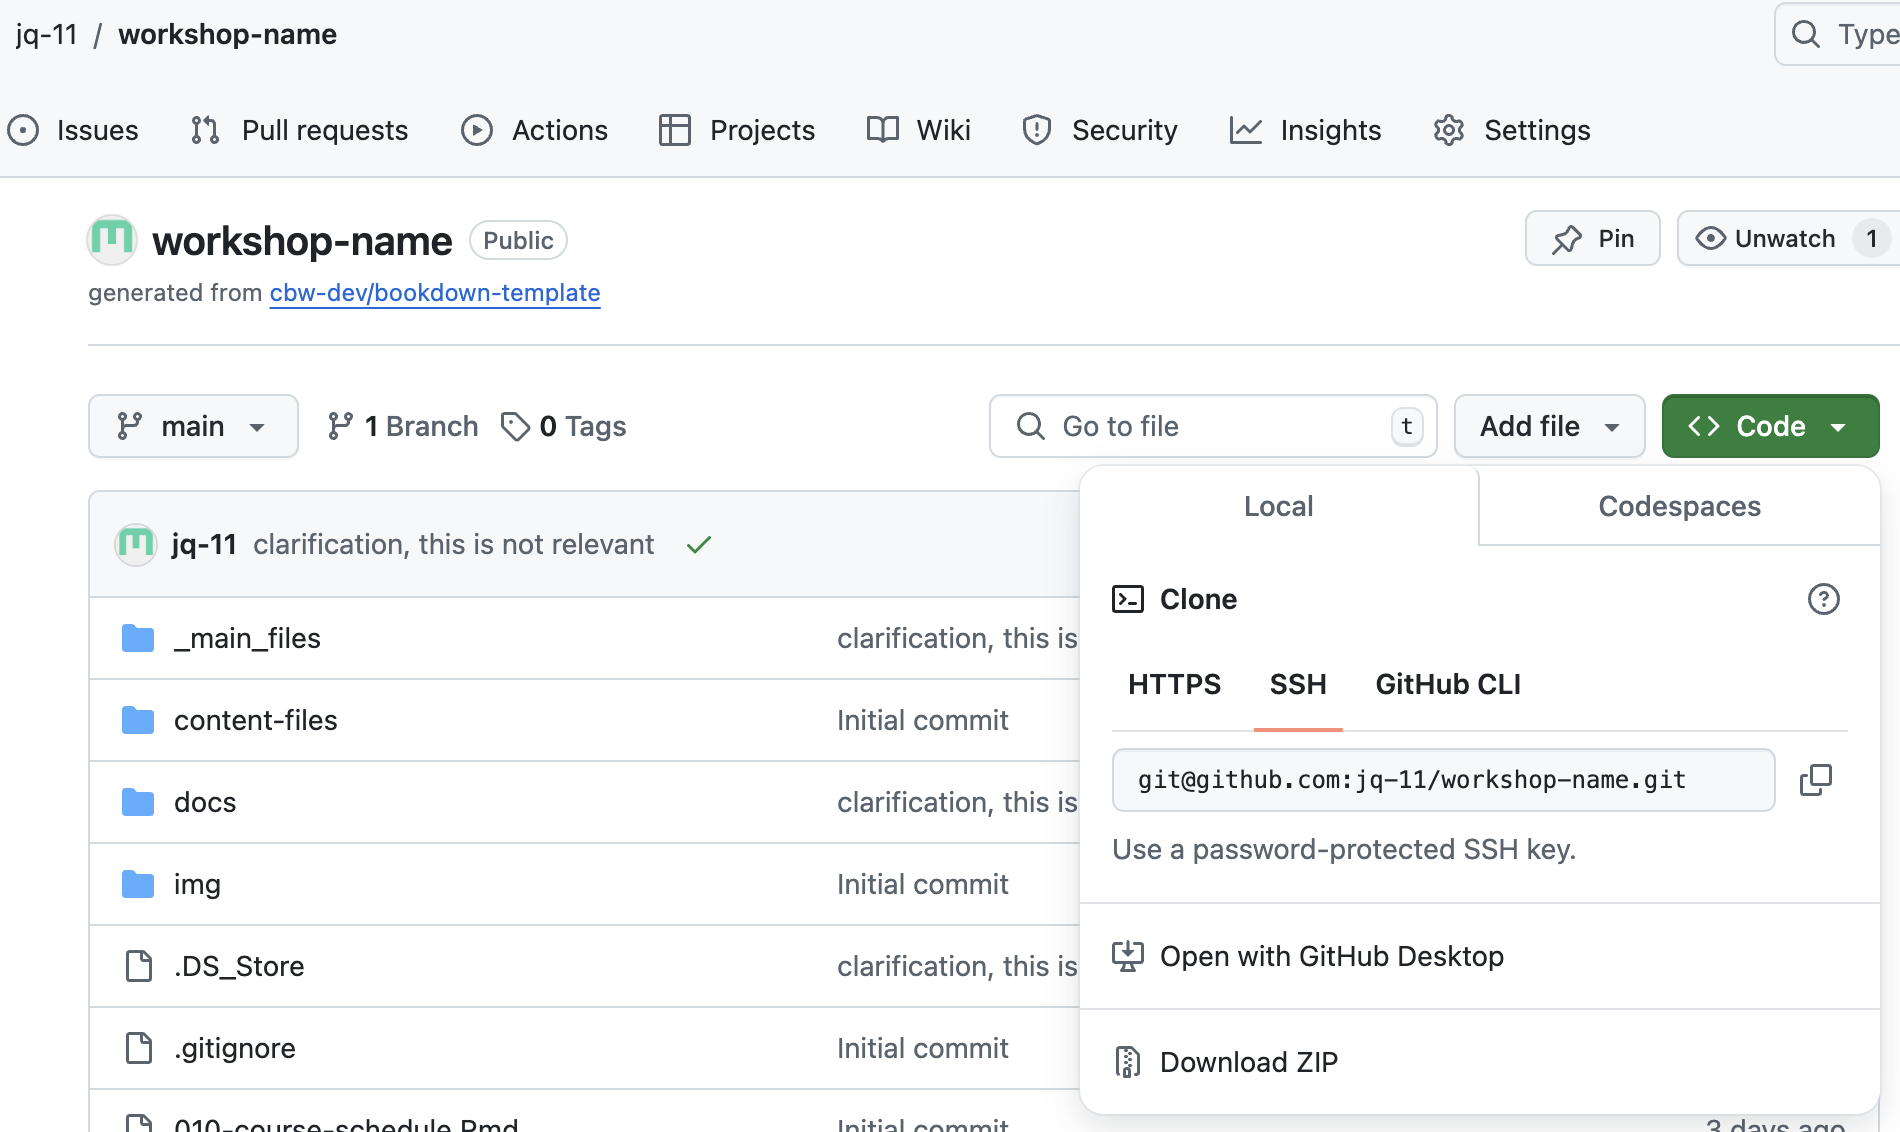
\includegraphics{img/git-instruct/copy-ssh.png}\\
  \item
    \textbf{Edit} and \textbf{run the following command} in Terminal/PowerShell/Command Prompt, within the folder you want the workshop folder to be in. (Recall that we navigated there in step 1.)
  \end{enumerate}

  \begin{redbox}

  \begin{center}
  \textbf{EDIT THE FOLLOWING COMMAND!}

  \end{center}

  You can essentially type ``git clone'' and then paste the SSH url, and then hit enter. Below, you must delete the entire ``{git@}github.com:bioinformaticsdotca/{[}YOUR WORKSHOP NAME{]}.git'' text, and replace it with the text you copied.

  \end{redbox}

\begin{verbatim}
git clone git@github.com:bioinformaticsdotca/[YOUR WORKSHOP NAME].git
\end{verbatim}
\item
  You should be ready to go! With your given permissions, you should be able to git push (put your local edits on GitHub) and git pull (pull edits on GitHub to your local computer) fine!
\end{enumerate}

\begin{bluebox}

\begin{center}
\textbf{Git Version Control Tip!}

\end{center}

Consider having only one team member (or perhaps your RC) make git pushes or control pull requests. To avoid merge conflicts, designate 1 team member to control actual changes to your workshop repo. Other team members can fork or create branches, and create a pull request that the designated team member can check and overlook.

\end{bluebox}

But what do any of these files mean? Which ones do I edit? Which ones shouldn't I edit? How do I open this in RStudio? And how exactly is a page made from all these files??? It's time for you to go to the next page :D

\subsection{Oops, I Git Cloned the Wrong Repository and I Want to Delete it from my Local Computer!}\label{oops-i-git-cloned-the-wrong-repository-and-i-want-to-delete-it-from-my-local-computer}

That's ok! To delete the entire local repository and the folder itself, run the following command:

\begin{verbatim}
rm -fr folder-path
\end{verbatim}

where ``folder-path'' is a file address to the git cloned folder/repository that you want to delete.

\chapter{So What Do These Files Mean?}\label{file-explanation}

Ok now we have our workshop locally (on our computer), which is made up of all these files and folders?

Before we dive deep into what to do with these folders, let's explore how bookdown actually works and how to understand RStudio.

\section{Bookdown Simple Explanation}\label{bookdown-simple-explanation}

Here is a general summary of how Bookdown creates html websites from .Rmd files.

Essentially, knitr renders and runs all the code, and the outputs are converted into markdown. After knitr, we essentially have a bunch of only markdown files.

Pandoc translates this markdown into html, so that we get a website! It can be helpful to know when and how these packages work, to help debug later on!

Now, let's figure out RStudio. Skip to \hyperref[file-setup]{file setup} if you already know how to use RStudio (and it's built in git control window).

\section{Opening Your Bookdown Project in RStudio}\label{opening-your-bookdown-project-in-rstudio}

Enter the folder you just git cloned using Finder/File Explorer, it should be titled ``{[}workshop-name{]}''. Right click on {[}workshop-name{]}.Rproj and press ``Open in RStudio''. There is only one file with this file extension. The .Rproj file is what you will open each time you want to work on this workshop! You must explicitly \textbf{open the .Rproj} file to build properly!

A RStudio window should open up and look something like the image below.
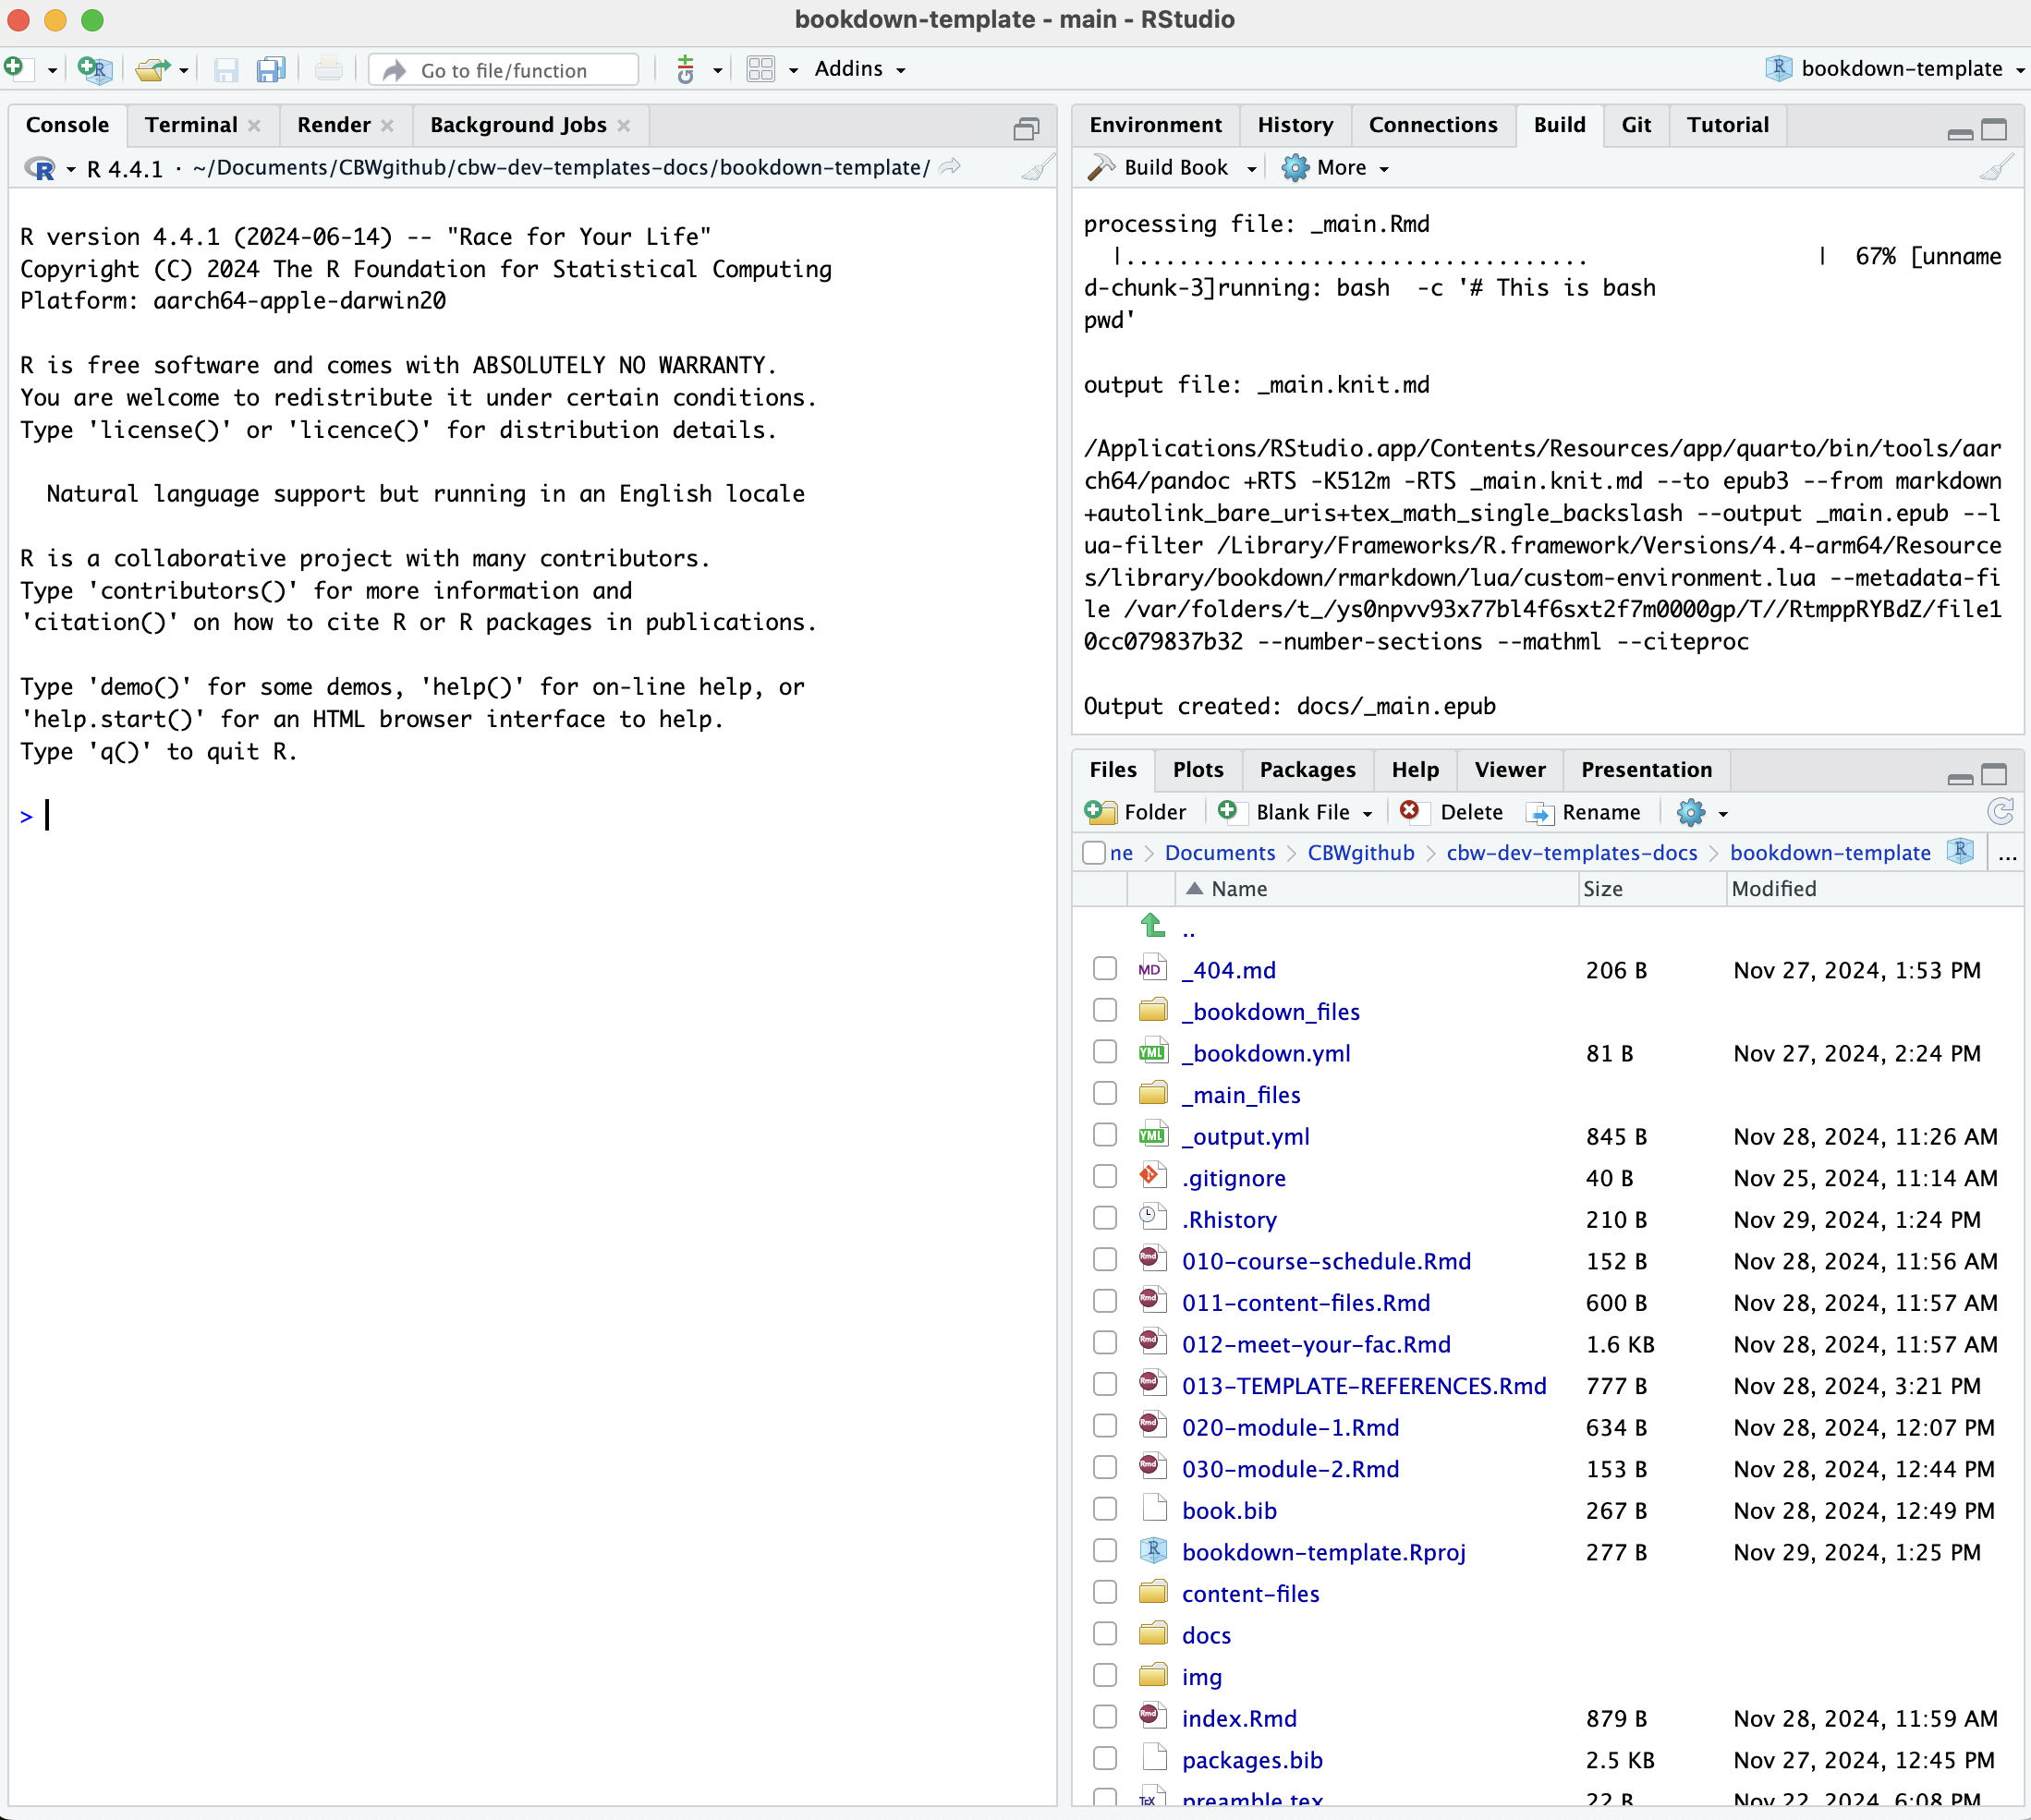
\includegraphics{img/files-and-build/newly-opened-RStudio.png}\\

\section{Explaining RStudio}\label{explaining-rstudio}

In the bottom right, we have all of our files and subfolders. These files will be explained \hyperref[file-setup]{below}. This window also contains helpful views, like ``Viewer'' and ``Plots''. We will touch on these later.

Try opening \texttt{index.Rmd}: a new pane will open in the top left that shows the contents of \texttt{index.Rmd}. This is where we will be editing our files! Notice, the ``Knit'' button.

In the bottom left, we have our console and other debug related windows (such as terminal!). Any code we run will appear in the console. We can access the terminal (just like editing in the Terminal app) under the ``Terminal'' tab.

In your top right, we have a different window with more different views. The most relevant windows to us are the ``Build'' and the ``Git'' windows.

\begin{quote}
No ``Git'' Window?

Try closing (and maybe even restarting RStudio) and then reopening it. A ``Git'' tab should appear to the right of the ``Build'' tab and to the left of the ``Tutorial'' tab.
\end{quote}

\section{Build the Book}\label{build-the-book}

Try pressing ``Build Book'' within the ``Build'' window. Your build window is going to fill up with text, and soon, a website is going to pop-up as your new window. This is the website you will be editing to create your workshop!

\begin{quote}
Note: If it's your first time building, you may have to approve some downloads and installations, like we did in \hyperref[get-started]{Getting Started}!
\end{quote}

By building the book, \textbf{all} of these files were compiled and converted to .html files, that create a website. Each time we make local changes to our files and we want them to appear in our website, we need to rebuild the book. Note that each time we build our book, the files we edited will be saved first (we don't have to save before building!).

\begin{quote}
Note: By default, RStudio will choose to build ``All Formats'':
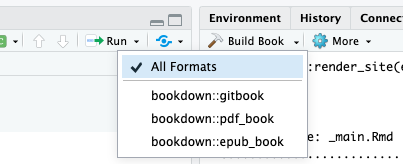
\includegraphics{img/files-and-build/build-book-options.png}\\
You can choose to only produce a gitbook (the first option). This can be helpful if you are encountering errors claiming that ``bookdown::render\_book() failed to render the output format `bookdown::pdf\_book'/bookdown::epub\_book'''. Additionally, not producing all output formats can decrease your build time significantly! (However, not being able to produce the other ouputs may suggest there is an underlying bug. It is ideal to be abble to produce all outputs.)
\end{quote}

\subsection{Other Ways to Build Your Book}\label{other-ways-to-build-your-book}

\begin{enumerate}
\def\labelenumi{\arabic{enumi}.}
\tightlist
\item
  Build the book from the R console:
\end{enumerate}

\begin{Shaded}
\begin{Highlighting}[]
\NormalTok{bookdown}\SpecialCharTok{::}\FunctionTok{render\_book}\NormalTok{()}
\end{Highlighting}
\end{Shaded}

\begin{enumerate}
\def\labelenumi{\arabic{enumi}.}
\setcounter{enumi}{1}
\tightlist
\item
  Press the keyboard buttons: \texttt{cmd\ +\ shift\ +\ B} (macOS) OR \texttt{ctrl\ +\ shift\ +\ B} (windows)
\end{enumerate}

\subsection{Knit Your Book}\label{knit-your-book}

Building can take a long time. If you are editing just one file, you can press the ``Knit'' button that is at the top of the window with your file. This will run the code in the page, and show you what that page would look like in the website (as well as saving that file).

\begin{quote}
Note: Other pages in your website will not update.
\end{quote}

\begin{quote}
A quicker way to knit is using the keboard controls

\texttt{cmd\ +\ shift\ +\ K} (macOS) OR \texttt{ctrl\ +\ shift\ +\ K} (Windows)
\end{quote}

\subsubsection{Knit VS Build}\label{knit-vs-build}

Building creates the website using \textbf{ALL} the .Rmd (and other) files. This is why it takes so long. Knitting creates/updates \textbf{only} the .Rmd file you're currently working in and reruns your code. (Note: You can't knit a non-.Rmd file!)

Before pushing to GitHub, it is a good idea to build, in case of faulty links or small bugs that occur if you only knit or preview.

\subsection{Preview Your Book}\label{preview-your-book}

If you want live updates to your changes, you can preview the page as you edit the book when you save individual .Rmd files. You can start the server in a work session by using the RStudio add-in ``Preview book'', or from the R console (in the bottom left window):

\begin{Shaded}
\begin{Highlighting}[]
\NormalTok{bookdown}\SpecialCharTok{::}\FunctionTok{serve\_book}\NormalTok{()}
\end{Highlighting}
\end{Shaded}

But which files do we edit? Well alas, it's time to discuss the file setup.

\section{File Setup Explanation}\label{file-setup}

Recall:

Hence, all the .Rmd files create a page in the produced website! To create more pages, you will be creating more .Rmd files.

Here is a tree diagram of the bookdown template setup. (Note that this mimics how RStudio displays the files, if your RStudio shows these template files in a different order, right click your file window and press ``Reload'')

\begin{quote}
\textbf{Note:} only relevant files or files you might be concerned about are explained in blue. If there is no explanation, you can safely assume you do not have to worry about it.
\end{quote}

\begin{Shaded}
\begin{Highlighting}[]
\ExtensionTok{bookdown{-}template}
\ExtensionTok{├──}\NormalTok{ \_404.md }\CommentTok{\# This becomes your 404 page. This is the only file that can become a page that can also be either a .md or .Rmd file!}
\ExtensionTok{├──}\NormalTok{ \_bookdown.yml }\CommentTok{\# a config file, you most likely won\textquotesingle{}t have to edit it unless you want additional configuration settings}
\ExtensionTok{├──}\NormalTok{ \_bookdown\_files}
\ExtensionTok{├──}\NormalTok{ \_main\_files}
    \ExtensionTok{└──}\NormalTok{ ... }\CommentTok{\# [in case of confusion: image and pdf output files]}
\ExtensionTok{├──}\NormalTok{ \_output.yml }\CommentTok{\# a config file, RC/workshop team will have to edit a few things (the workshop name, sponsor images, repo link)}
\ExtensionTok{├──}\NormalTok{ .gitignore}
\ExtensionTok{├──}\NormalTok{ .Rhistory}
\ExtensionTok{├──}\NormalTok{ 010{-}course{-}schedule.Rmd }\CommentTok{\# {-}{-}\textgreater{} "Course Schedule" section}
\ExtensionTok{├──}\NormalTok{ 011{-}content{-}files.Rmd }\CommentTok{\# {-}{-}\textgreater{} "Pre{-}workshop Materials" and "Computing Setup \& Downloads" section}
\ExtensionTok{├──}\NormalTok{ 012{-}meet{-}your{-}fac.Rmd }\CommentTok{\# {-}{-}\textgreater{} "Meet Your Faculty" section}
\ExtensionTok{├──}\NormalTok{ 020{-}module{-}1.Rmd }\CommentTok{\#{-}{-}\textgreater{} "Module 1", "Lecture, and "Lab" section}
\ExtensionTok{├──}\NormalTok{ 030{-}module{-}2.Rmd}
\ExtensionTok{├──}\NormalTok{ README.md }\CommentTok{\# README file that has some helpful explanations, consider reading this before starting to edit (along with this documentation!)}
\ExtensionTok{├──}\NormalTok{ book.bib }\CommentTok{\# citation file}
\ExtensionTok{├──}\NormalTok{ bookdown{-}template.Rproj }\CommentTok{\# always open this file in RStudio, opening this helps bookdown understand what to build}
\ExtensionTok{├──}\NormalTok{ content{-}files }\CommentTok{\# store all files from your modules here (ex. data sets, empty code worksheets)}
    \ExtensionTok{└──}\NormalTok{ sample{-}pdf.pdf}
\ExtensionTok{├──}\NormalTok{ docs}
    \ExtensionTok{└──}\NormalTok{ ... }\CommentTok{\# html files \& other generated content}
\ExtensionTok{├──}\NormalTok{ img }\CommentTok{\# folder where you should store all your images}
    \ExtensionTok{├──}\NormalTok{ bioinformatics.ca{-}logo.svg }
    \ExtensionTok{├──}\NormalTok{ faculty }\CommentTok{\# store all images of faculty in this folder}
        \ExtensionTok{├──}\NormalTok{ michelle{-}brazas.jpg}
        \ExtensionTok{└──}\NormalTok{ nia{-}hughes.jpeg}
    \ExtensionTok{├──}\NormalTok{ favicon.ico}
    \ExtensionTok{└──}\NormalTok{ sponsors }\CommentTok{\# store all sponsor logos/titles in this folder}
         \ExtensionTok{└──}\NormalTok{ Your{-}Sponsor{-}Here.svg}
\ExtensionTok{├──}\NormalTok{ index.Rmd }\CommentTok{\# landing page {-}{-}\textgreater{} "Welcome" section}
\ExtensionTok{├──}\NormalTok{ packages.bib }\CommentTok{\# R generated citation file}
\ExtensionTok{├──}\NormalTok{ preamble.tex}
\ExtensionTok{└──}\NormalTok{ style.css }\CommentTok{\# css styling options are defined here {-} feel free to add your own styling features}
\end{Highlighting}
\end{Shaded}

\subparagraph*{\texorpdfstring{ \_output.yml \& \_bookdown.yml }{ \_output.yml \& \_bookdown.yml }}\label{output.yml-_bookdown.yml}
\addcontentsline{toc}{subparagraph}{ \_output.yml \& \_bookdown.yml }

2 important files are the \texttt{\_output.yml} files and the \texttt{\_bookdown.yml} files. They help tell bookdown what we want and what to do, especially when making our website.

You will only have to edit \_output.yml a bit. The \_output.yml file creates the table of contents/sidebar you see on the left of the workshop. It is written in HTML, which is why it looks so different. There are 3 things either the RC or the workshop team will need to do:

\begin{enumerate}
\def\labelenumi{\arabic{enumi}.}
\item
  Change the workshop name: {[}YOUR WORKSHOP NAME{]} on line 7.
\item
  Add your sponsors: Replace ``Your-Sponsor-Here.svg'' with the file name of your sponsors name/logo. Remember to place these files inside the ./img/sponsors/ folder.
\item
  Replace your workshop repo edit link. This allows users to suggest edits to your work on GitHub. Follow these instructions (they are also provided in the template).

  \begin{enumerate}
  \def\labelenumii{\arabic{enumii}.}
  \tightlist
  \item
    Go to your index.Rmd page on GitHub, Copy and paste the link to it.
  \item
    Copy and paste the link to it, excluding the ``index.Rmd'' ending.
  \item
    Add \texttt{/\%s} to the ending.
  \item
    Replace the above link.
  \end{enumerate}
\end{enumerate}

\subparagraph*{\texorpdfstring{ Organizing the Table of Contents }{ Organizing the Table of Contents }}\label{organizing-the-table-of-contents}
\addcontentsline{toc}{subparagraph}{ Organizing the Table of Contents }

The order of the sidebar is completely dependent on the alphabetical order of the files (see your bottom right window pane! The order is generally the same as the order shown in the RStudio file window pane. If not, right click the window and press ``Reload''). Our template has numbering first, to help ease our understanding and organization of files. The only file without this is \texttt{index.Rmd}, since as the landing page we can not change the file name.

\subparagraph*{\texorpdfstring{ index.Rmd }{ index.Rmd }}\label{index.rmd}
\addcontentsline{toc}{subparagraph}{ index.Rmd }

The only .Rmd that must have some configuration details is the landing page: \textbf{index.Rmd}. This is what fills up the beginning of the index.Rmd file, surrounded by the -\/-\/-, which tells bookdown the configuration information.

\textbf{Follow the instructions in the template's index.Rmd file - you must fill in the title, author, date and url.} The description, cover-image and github-repo can be changed, but aren't mandatory.

\subparagraph*{\texorpdfstring{ .Rmd Files }{ .Rmd Files }}\label{rmd-files}
\addcontentsline{toc}{subparagraph}{ .Rmd Files }

Let's move on to discussing the breakdown of the .Rmd files. Each new page is defined by a new header, which starts with \texttt{\#}, each sub-header has increasingly more \texttt{\#} symbols (\#\#, \#\#\#, and more all create smaller sub-headers). A ``main'' header only has 1 \texttt{\#} symbol. These headers define new pages, as well as the title in the sidebar referring to that page.

Hence, if we have multiple ``main'' headers in 1 .Rmd file, 1 .Rmd file will encode multiple pages. Try to have only 1 single \# as a header on one page! (You may get warnings otherwise).

However, if a new file only has sub-headers (2 \texttt{\#} or more), the sub-header will appear on the page that was defined by the previous .Rmd file (in alphabetical order - see the order of the ``File'' window pane).

In our template, we want the introduction material to appear on the same page. Hence, the introduction files (other than 020-course-schedule.Rmd, which starts the page) all only have sub-headers.

\emph{Note:} Due to this, you may receive this warning:

\begin{quote}
Warning message:
In split\_chapters(output, gitbook\_page, global\_numbering, split\_by, :
You have 6 Rmd input file(s) but only 4 first-level heading(s). Did you forget first-level headings in certain Rmd files?
\end{quote}

You can ignore this warning message!

\subparagraph*{\texorpdfstring{ How to Create a New File }{ How to Create a New File }}\label{how-to-create-a-new-file}
\addcontentsline{toc}{subparagraph}{ How to Create a New File }

You can create new files anywhere. You should only be making new website pages, so you should also only be making .Rmd files. (Creating new .md files in hopes of making a new page usually ends up with weird bugs, stick to .Rmd files).

\begin{enumerate}
\def\labelenumi{\arabic{enumi}.}
\tightlist
\item
  Under the ``Files'' tab of the lower right window pane, there are many options to modify your files. You can use these buttons instead of your File Explorer. Click ``New Blank File''.
\item
  Click the second dropdown option: R Markdown
\item
  Give your file a unique name that matches CBW's Bookdown template file naming convention. That is, ``0XX-{[}description{]}.Rmd''. Decide what X should be depending on where you want the page to show up on your sidebar. Name your file a short but descriptive name, with hyphens (-) to split up words.
\item
  Start editing your new file in the upper left window!
\end{enumerate}

\subparagraph*{\texorpdfstring{ 404 Page }{ 404 Page }}\label{page}
\addcontentsline{toc}{subparagraph}{ 404 Page }

That being said, there is one file that can be a markdown (.md) file: the \_404.(R)md file. If website user goes to a webpage that belongs to our website but no longer exists, they will get this 404 page instead. Put links to your landing page for your workshop or the bioinformatics.ca homepage here!

\subparagraph*{\texorpdfstring{ CBW Organization Folders }{ CBW Organization Folders }}\label{cbw-organization-folders}
\addcontentsline{toc}{subparagraph}{ CBW Organization Folders }

We want our workshops to be easy to navigate and understand. Hence, images or files that are required for your lessons should be placed in \texttt{./img/} and \texttt{./content-files/} respectively. Within these files, try creating sub-folders within these folders to help organize groups of files. For example, if you have a bunch of data sets, try creating a ``datasets'' folder within \texttt{./content-files/}.

Subfolders already exist in \texttt{./img}: \texttt{./img/faculty/} and \texttt{./img/sponsors/}. Fill these with photos of your faculty and images of the names'/logos' of your sponsors, respectfully!

\subparagraph*{\texorpdfstring{ Bookdown's Wesbite Building Folders }{ Bookdown's Wesbite Building Folders }}\label{bookdowns-wesbite-building-folders}
\addcontentsline{toc}{subparagraph}{ Bookdown's Wesbite Building Folders }

Bookdown makes some folders to store .html files, among other files that help create the website. Hence, you should not (need to) touch:

\begin{itemize}
\tightlist
\item
  \_bookdown\_files
\item
  \_main\_files
\item
  docs
\end{itemize}

\begin{quote}
\textbf{Debugging Tip}: If you do get an error that seems like it's coming from one of these files, there was probably an error that resulted from bookdown not being able to process something. Double check that your syntax, formatting, file names and related files are correct.
\end{quote}

\begin{quote}
\textbf{Debugging Tip 2}: Each time we build, we produce a ``docs'' folder. If we have already built once, we just add new files to it. HTML files that were produced from .Rmd that were deleted are not removed. Hence, if you see errors from files that no longer exist in your root project folder, try deleting the whole docs folder, and rebuilding.
\end{quote}

\section{Push to GitHub via RStudio}\label{push-to-github-via-rstudio}

Now, we know what our files mean and how to edit them. How do we get this onto GitHub? We can write git commands into our Terminal/Command Prompt, or alternatively (and more easily), RStudio has a built-in git interface.

Now, we will be able to see a Git window in the top right. Click ``Git'' to open this window.

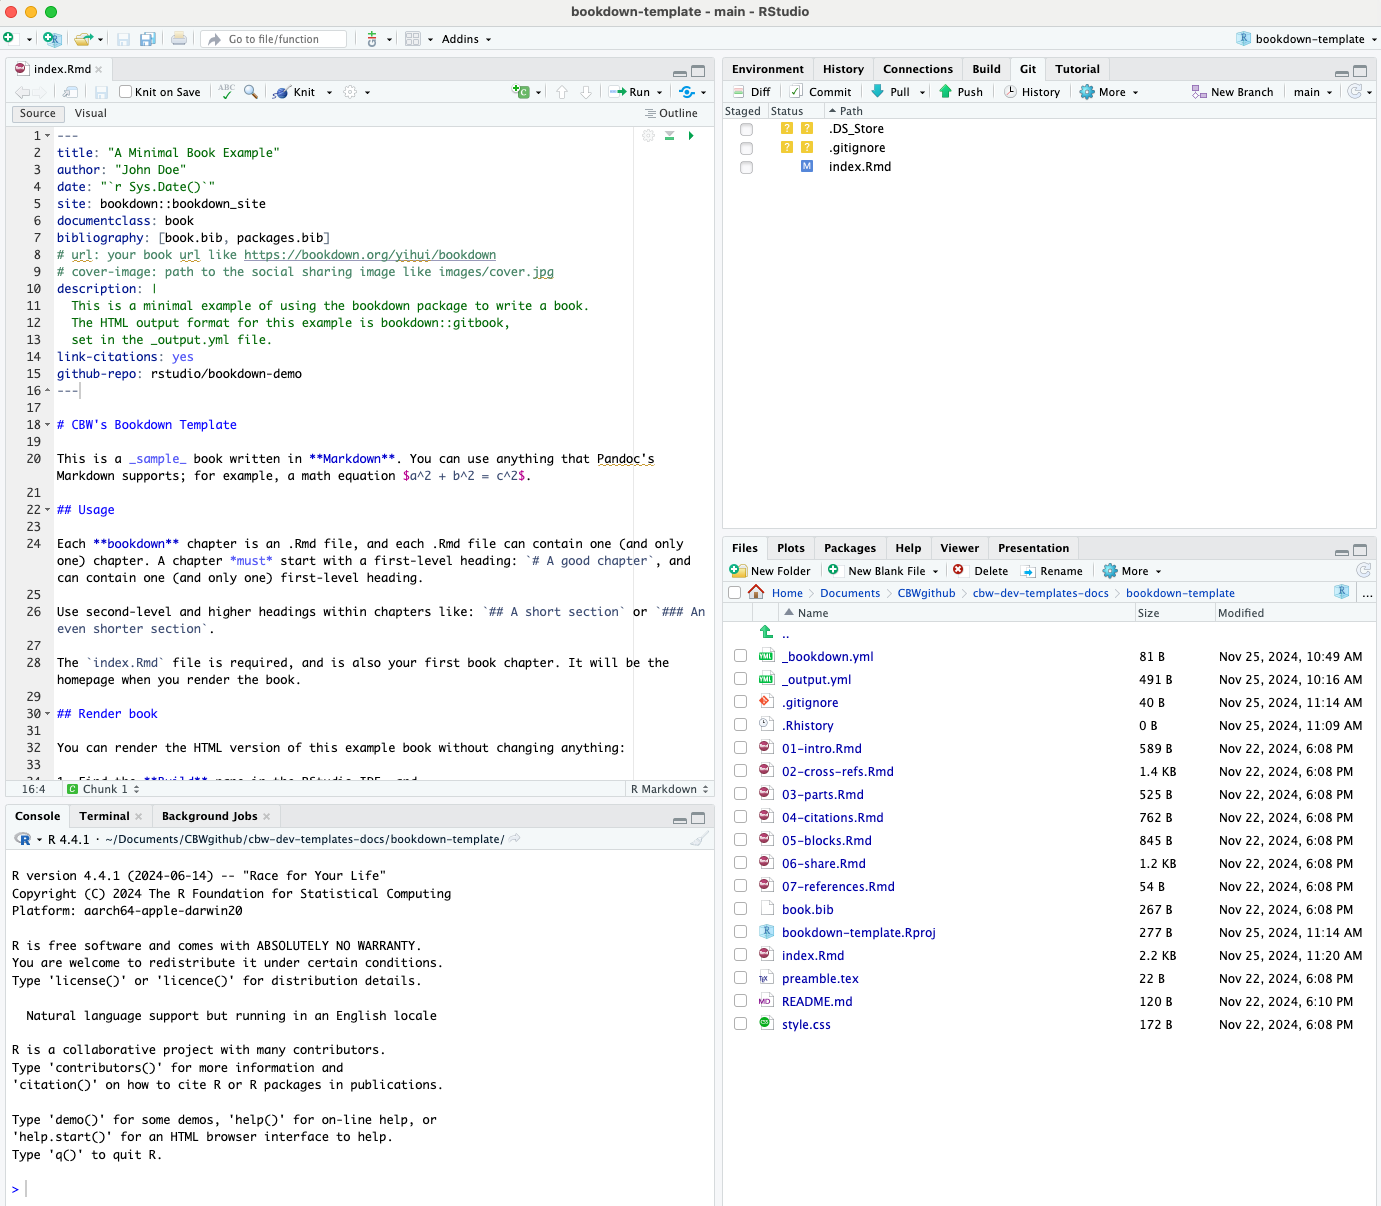
\includegraphics{img/git-instruct/RStudio-with-git-window-open.png}\\

Let's say we only edited \texttt{index.Rmd}, now we see the newly edited files. Changed files that need to be updated on GitHub will show up in this window, like how \texttt{index.Rmd} is seen above. (Do not worry too much about \texttt{.DS\_Store} and \texttt{.gitignore} do.) Let's try to push this change to GitHub.

\begin{enumerate}
\def\labelenumi{\arabic{enumi}.}
\item
  Select all the edited files.

  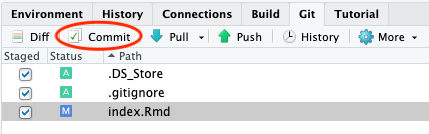
\includegraphics{img/git-instruct/git-window-selected-items.png}\\
\item
  Then, click the Commit button, which appears above your selected items. A window pane will appear (shown below).

  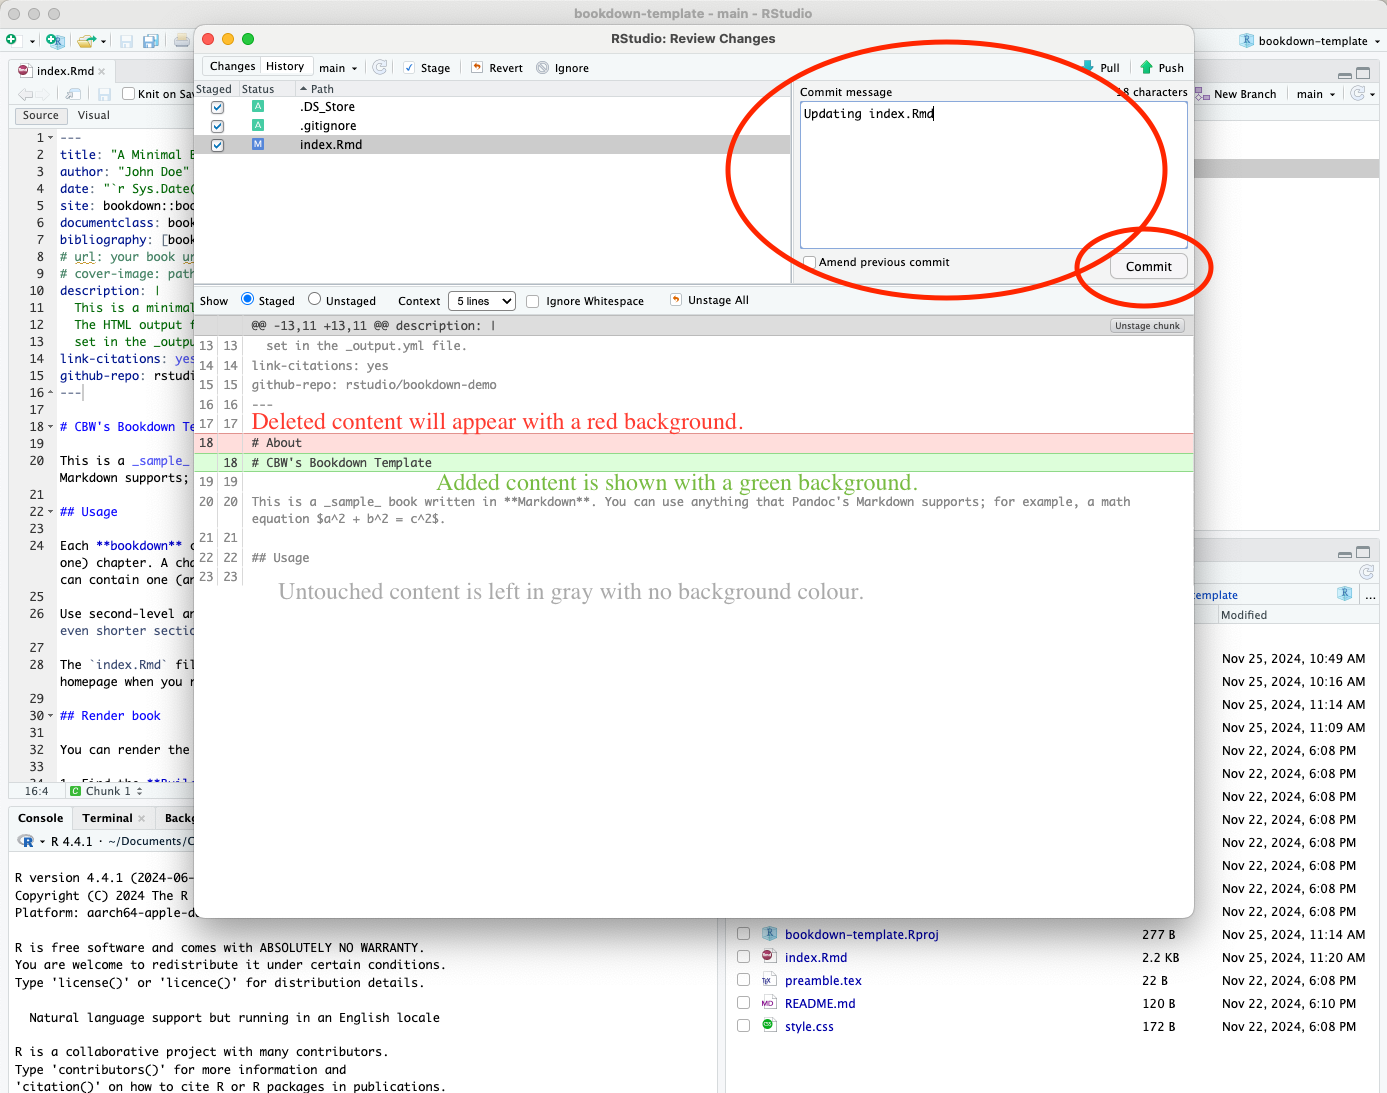
\includegraphics{img/git-instruct/git-commit-window.png}\\
\item
  Add a commit message in the corresponding box, and then press commit below it.
\item
  A new window will show up, detailing your updates. Close this window and then press \textbf{Push} to push your updates to GitHub.

  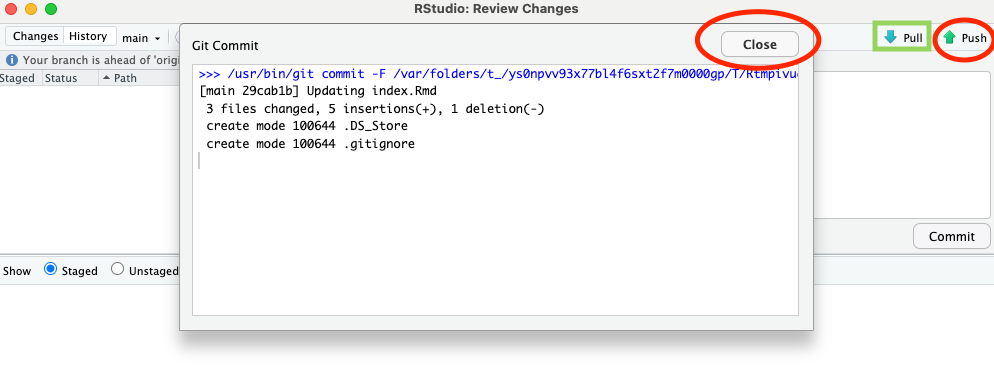
\includegraphics{img/git-instruct/git-window-post-commit.png}\\
\end{enumerate}

Now, we're done! We should see the updates on GitHub now. Also note, if we ever want to pull updates from GitHub, there is also a \textbf{Pull} button in the Git window within RStudio!

\emph{Git pushing} puts your edits onto GitHub, \emph{git pulling} takes the edits make on GitHub, and brings them to your local computer. For example, if one of your workshop team members made an edit, you want to have that edit on your computer before you start editing! It's a good idea to do this (git pull - upper right window, ``Pull'' button) before you start editing, in case somehow your edits conflicts with their edits.

Git pushing will automatically update the website, you can see the updates and progress in the actions window we saw previously. (Check out your website on the web once it's done deploying!)

\chapter{Formatting Your Content - Markdown}\label{formatting}

Now we know which files to edit, but how can we edit these files? How do we format our text, links, headers, \ldots?

\section{Visaul R Markdown}\label{visual-r-md}

All our files are made up of code and markdown syntax, that becomes formatted into our website. However, if you do not feel comfortable using Markdown (or you just want an easier way to write your pages), see this guide on using Visual R Markdown.

It can be significantly easier to use Visual R Markdown, especially for those who are used to working in Google Docs!

If you want to use Markdown, a basic syntax guide is provided below!

\begin{quote}
Is this not enough for you?

Bookdown has thorough documentation for specific elements, customizations, and further explanations. For simple elements, everything is provided below. However, there are many more possibilities with Bookdown! Click here to read more!
\end{quote}

\begin{quote}
\textbf{IMPORTANT NOTE}: Now that you're straying away from CBW's Bookdown template, there's a chance you may run into errors. See \hyperref[help]{this page} for help!
\end{quote}

\section{Chapters}\label{chapters}

As mentioned earlier, headers are defined by a \# before the title. Subheaders get increasingly more nested as add more \# symbols before it. For example,

\begin{verbatim}
# Hello
\end{verbatim}

would create a chapter title. Since there is only one \texttt{\#} symbol, this would also create a new page. Again, try to keep only one chapter title per .Rmd file.

\begin{verbatim}
## Subheader
\end{verbatim}

\section{Subheader}\label{subheader}

This is what a subheader would look like.

\begin{verbatim}
### Subheader
\end{verbatim}

\subsection{Subheader}\label{subheader-1}

This is what a subheader with 3 \texttt{\#} symbols would look like. You can add as many \texttt{\#} symbols as you would like! There is also no limit to the the number of subheaders you can have.

\subsection*{An unnumbered subheader}\label{an-unnumbered-subheader}
\addcontentsline{toc}{subsection}{An unnumbered subheader}

Chapters and sections are numbered by default. To un-number a heading, add a \texttt{\{.unnumbered\}} or the \texttt{\{-\}} at the end of the heading. For example, the above subheader was written like this:

\begin{verbatim}
### An unnumbered subheader {-}
\end{verbatim}

\section{Parts}\label{parts}

Notice how index.Rmd in our CBW Bookdown template has \texttt{\#\ (PART)\ Introduction\ \{-\}} (followed by \texttt{\#\ Welcome}). This creates the ``Introduction'' section on the sidebar.

There are already 2 main parts in the template: the introduction and modules sections.

If you want to add more parts, simply paste this: \texttt{\#\ (PART)\ {[}Part\ Title{]}\ \{-\}} into a new .Rmd file, at the top of the file, before the main \texttt{\#\ header} for that page/file.

\textbf{Note}: If you would like to have a un-numbered part: Use this syntax: \texttt{\#\ (PART\textbackslash{}*)\ {[}Part\ Title{]}\ \{-\}}

\textbf{Another Note}: A similar un-numbered part is called an ``Appendix'' and Bookdown. Like a part, paste \texttt{\#\ (APPENDIX)\ {[}Appendix\ Name{]}\ \{-\}} it above the ``main'' header you would like it to be before. All subsequent headers will be described via letters rather than numbers. (If your following headers are un-numbered, an Appendix looks the same as an un-numbered part).

\section{Text Formatting}\label{text-formatting}

Before we go ahead with much more formatting possibilities, let's get the basics of markdown formatting options for basic text. (Tip: There are many resources online that can help give more information!)

\subsection*{Bold}\label{bold}
\addcontentsline{toc}{subsection}{Bold}

\begin{Shaded}
\begin{Highlighting}[]
\NormalTok{**bolded text**}
\end{Highlighting}
\end{Shaded}

\textbf{bolded text}

\subsection*{Italics}\label{italics}
\addcontentsline{toc}{subsection}{Italics}

\begin{Shaded}
\begin{Highlighting}[]
\NormalTok{*italicized text*}
\end{Highlighting}
\end{Shaded}

\emph{italicized text}

\subsection*{Subscript}\label{subscript}
\addcontentsline{toc}{subsection}{Subscript}

\begin{verbatim}
H~2~O
\end{verbatim}

H\textsubscript{2}O

\subsection*{Superscript}\label{superscript}
\addcontentsline{toc}{subsection}{Superscript}

\begin{verbatim}
Na^+^
\end{verbatim}

Na\textsuperscript{+}

\subsection*{Footnotes}\label{footnotes}
\addcontentsline{toc}{subsection}{Footnotes}

\texttt{\^{}{[}{]}} is the formatting for a footnote. For example

\begin{verbatim}
Here is a footnote: ^[This is a footnote.].
\end{verbatim}

Here is a footnote: \footnote{This is a footnote.}.

(Scroll to the bottom of this page to see it.)

\subsection*{Horizontal Line}\label{horizontal-line}
\addcontentsline{toc}{subsection}{Horizontal Line}

\begin{verbatim}
---
\end{verbatim}

\begin{center}\rule{0.5\linewidth}{0.5pt}\end{center}

\subsection*{Blockquote}\label{blockquote}
\addcontentsline{toc}{subsection}{Blockquote}

\begin{Shaded}
\begin{Highlighting}[]
\AttributeTok{\textgreater{} blockquote}
\AttributeTok{\textgreater{}}
\AttributeTok{\textgreater{} {-}{-}{-} someone who blockquotes}
\end{Highlighting}
\end{Shaded}

\begin{quote}
blockquote

--- someone who blockquotes
\end{quote}

You can put emojis to help these standout! For example:

\begin{quote}
⚠️ \textbf{Warning:} Do not push the big red button.
\end{quote}

\subsection*{Unordered List}\label{unordered-list}
\addcontentsline{toc}{subsection}{Unordered List}

\begin{Shaded}
\begin{Highlighting}[]
\SpecialStringTok{{-} }\NormalTok{unordered}
\SpecialStringTok{  {-} }\NormalTok{list}
\SpecialStringTok{    {-} }\NormalTok{element}
\SpecialStringTok{{-} }\NormalTok{cool!}
\end{Highlighting}
\end{Shaded}

\begin{itemize}
\tightlist
\item
  unordered

  \begin{itemize}
  \tightlist
  \item
    list

    \begin{itemize}
    \tightlist
    \item
      element
    \end{itemize}
  \end{itemize}
\item
  cool!
\end{itemize}

\begin{quote}
Warning: Bookdown currently can not render Markdown to-do lists properly. Alternatively, use \hyperref[use-html]{this tip} instead!
\end{quote}

\subsection*{Ordered List}\label{ordered-list}
\addcontentsline{toc}{subsection}{Ordered List}

\begin{Shaded}
\begin{Highlighting}[]
\SpecialStringTok{1. }\NormalTok{First item}
\SpecialStringTok{    1. }\NormalTok{a }\CommentTok{\textless{}!{-}{-} For nesting inside a list, put 2 tabs before the element {-}{-}\textgreater{}}
\SpecialStringTok{    2. }\NormalTok{b}
\SpecialStringTok{2. }\NormalTok{Second item}
\SpecialStringTok{3. }\NormalTok{Third item}
\end{Highlighting}
\end{Shaded}

\begin{enumerate}
\def\labelenumi{\arabic{enumi}.}
\tightlist
\item
  First

  \begin{enumerate}
  \def\labelenumii{\arabic{enumii}.}
  \tightlist
  \item
    a

    \begin{enumerate}
    \def\labelenumiii{\arabic{enumiii}.}
    \tightlist
    \item
      c
    \item
      d
    \end{enumerate}
  \item
    b
  \end{enumerate}
\item
  Second
\item
  Third
\end{enumerate}

\subsection*{Code}\label{code}
\addcontentsline{toc}{subsection}{Code}

There are 2 ways to write code:

\begin{enumerate}
\def\labelenumi{\arabic{enumi}.}
\item
  \texttt{\textasciigrave{}code\textasciigrave{}} which looks like this: \texttt{code}
\item
  Or long pieces of code

\begin{verbatim}
```
1 + 1  # a line of code
```
\end{verbatim}

  which would render into the following on your website

\begin{verbatim}
1 + 1  # a line of code
\end{verbatim}
\end{enumerate}

Find more code options and information in the \hyperref[render-code]{How to Render Code} section.

\subsection*{Images}\label{images}
\addcontentsline{toc}{subsection}{Images}

The basic notation for a file is:

\begin{verbatim}
![Alt Text](img/.../...)\
\end{verbatim}

For example:

\begin{verbatim}
![bioinformatics.ca logo](img/bioinformatics.ca-logo.jpg)\
\end{verbatim}


\includegraphics{img/bioinformatics.ca-logo.jpg}\\

Note: Markdown does not actually require the backslash ``\textbackslash{}''. However, since Bookdown uses Pandoc, we should add a backslash so that the alternative text does not become a caption for the image. This occurs when the image is not directly following or followed by text. \href{https://pandoc.org/MANUAL.html\#extension-implicit_figures}{Here} is where it's discussed in the Pandoc documentation!

\begin{quote}
Note: Before adding the ``\textbackslash{}'', Bookdown will show you the image that you are referring to (double-click the file address link) and it will remain on screen, within your .Rmd file. \emph{You can use this to double check the file address is correct.} After adding the ``\textbackslash{}'', you can double-click to check the file address is pointing to the right image (and it should hover below), but it will not remain on screen.
\end{quote}

\subsection*{Links}\label{links}
\addcontentsline{toc}{subsection}{Links}

Links to a webpage are as follows:

\begin{verbatim}
[Text you want to hyperlink](website link)
\end{verbatim}

For example,

\begin{verbatim}
Click [here](https://bioinformatics.ca/) to see the bioinformatics.ca main page!
\end{verbatim}

Click \href{https://bioinformatics.ca/}{here} to see the bioinformatics.ca main page!

\subsection*{Links to Other Pages/Sections within your Workshop Wesbite}\label{links-to-other-pagessections-within-your-workshop-wesbite}
\addcontentsline{toc}{subsection}{Links to Other Pages/Sections within your Workshop Wesbite}

Note these steps work for all headers, not just main (1 \texttt{\#}) headers:

\begin{enumerate}
\def\labelenumi{\arabic{enumi}.}
\tightlist
\item
  Label the heading: \texttt{\#\ Hello\ world\ \{\#nice-label\}}.

  \begin{itemize}
  \tightlist
  \item
    If you do not want to include a label, an automatic label is made: \texttt{\#\ Hello\ world} = \texttt{\#\ Hello\ world\ \{\#hello-world\}}.
  \item
    To label an un-numbered heading, use: \texttt{\#\ Hello\ world\ \{-\#nice-label\}} or \texttt{\{\#\ Hello\ world\ .unnumbered\}}.
  \end{itemize}
\item
  Next, reference the header in either 2 ways:

  \begin{itemize}
  \item
    If you want the number referring to your header, use: \texttt{\textbackslash{}@ref(label-name)}. For example:

    \begin{center}\rule{0.5\linewidth}{0.5pt}\end{center}

\begin{verbatim}
Please see Citations \\ref{citations}.
\end{verbatim}

    Please see Citations \ref{citations}.

    \begin{quote}
    Note: If you use this reference style for an unnumbered header, ``\textbf{??}'' will be used as the hyperlinked text.
    \end{quote}

    \begin{center}\rule{0.5\linewidth}{0.5pt}\end{center}
  \item
    If you want a customizable text hyperlink, use the following:

\begin{verbatim}
See the [Citations](#citations)!
\end{verbatim}

    See the \hyperref[citations]{Citations}!
  \end{itemize}
\end{enumerate}

\section{Citations}\label{citations}

Bookdown can help us create citations!

First, tell bookdown your sources!

\begin{Shaded}
\begin{Highlighting}[]
\CommentTok{\# automatically create a bib database for R packages}
\NormalTok{knitr}\SpecialCharTok{::}\FunctionTok{write\_bib}\NormalTok{(}\FunctionTok{c}\NormalTok{(}
  \FunctionTok{.packages}\NormalTok{(), }\StringTok{\textquotesingle{}bookdown\textquotesingle{}}\NormalTok{, }\StringTok{\textquotesingle{}knitr\textquotesingle{}}\NormalTok{, }\StringTok{\textquotesingle{}rmarkdown\textquotesingle{}}
\NormalTok{), }\StringTok{\textquotesingle{}packages.bib\textquotesingle{}}\NormalTok{)}
\end{Highlighting}
\end{Shaded}

This R code created a file called `packages.bib' (which is in the bookdown template) which is now filled with a bunch of bibliography entries. `book.bib' also has a manually entered bibliography entry. We must tell bookdown the files with bibliography information via the YAML \texttt{bibliography} key in index.Rmd. A bibliography entry essentially looks like:

\begin{Shaded}
\begin{Highlighting}[]
\SpecialCharTok{@}\NormalTok{type\{key,}
\NormalTok{  title }\OtherTok{=}\NormalTok{ \{...\},}
\NormalTok{  author }\OtherTok{=}\NormalTok{ \{...\},}
\NormalTok{  organization }\OtherTok{=}\NormalTok{ \{...\},}
\NormalTok{  year }\OtherTok{=}\NormalTok{ \{...\},}
\NormalTok{  url }\OtherTok{=}\NormalTok{ \{...\},}
\NormalTok{  ... }\CommentTok{\# see more possible fields at https://en.wikipedia.org/wiki/BibTeX}
\NormalTok{\}}
\end{Highlighting}
\end{Shaded}

\texttt{@type} refers to what type of source it is (ex. an article, book, manual, \ldots). \texttt{@key} refers to the name we refer to it by in in-text citations.

For example, \texttt{@R-bookdown} renders to \citet{R-bookdown}. Adding square brackets also adds parentheses once it's rendered: so \texttt{{[}@R-bookdown{]}} becomes \citep{R-bookdown}.

\textbf{Note:} The \hyperref[visual-r-md]{RStudio Visual Markdown Editor} can also make it easier to insert citations!

On any page that you cite, a \textbf{References} section will be autogenerated at the bottom of that page (scroll down)!

\textbf{Note:} When you cite, Bookdown also generates a citation list that it adds at the end of the last page of your website. However, Bookdown does not create a title, so on your very last page, add a \texttt{\#\ Reference} main header. (To avoid having a ``2 main headers in the same file'' error, you can create a new .Rmd file with only \texttt{\#\ Reference}).

\section{Equations}\label{equations}

Equations are written in latex. You can refer to them with a label you specify after writing it out!

\begin{Shaded}
\begin{Highlighting}[]
\KeywordTok{\textbackslash{}begin}\NormalTok{\{}\ExtensionTok{equation}\NormalTok{\}}
\SpecialStringTok{  f}\SpecialCharTok{\textbackslash{}left}\SpecialStringTok{(k}\SpecialCharTok{\textbackslash{}right}\SpecialStringTok{) = }\SpecialCharTok{\textbackslash{}binom}\SpecialStringTok{\{n\}\{k\} p\^{}k}\SpecialCharTok{\textbackslash{}left}\SpecialStringTok{(1{-}p}\SpecialCharTok{\textbackslash{}right}\SpecialStringTok{)\^{}\{n{-}k\}}
\SpecialStringTok{  (}\SpecialCharTok{\textbackslash{}\#}\SpecialStringTok{eq:binom) \# the label!}
\KeywordTok{\textbackslash{}end}\NormalTok{\{}\ExtensionTok{equation}\NormalTok{\}}
\end{Highlighting}
\end{Shaded}

\begin{equation}
  f\left(k\right) = \binom{n}{k} p^k\left(1-p\right)^{n-k}
  \label{eq:binom}
\end{equation}

You may refer to using \texttt{\textbackslash{}@ref(eq:binom)}, for example: \texttt{see\ Equation\ \textbackslash{}@ref(eq:binom)} becomes ``see Equation \eqref{eq:binom}''. The number \eqref{eq:binom} depends on the chapter and the number of equations already in said chapter (the first equation will be numbered \texttt{{[}chapter\ number{]}.1}).

\section{Theorems and Proofs}\label{theorems-and-proofs}

We also have specific syntax for theorems and proofs, for example, this code:

\begin{verbatim}
::: {.theorem #tri}
For a right triangle, if $c$ denotes the *length* of the hypotenuse
and $a$ and $b$ denote the lengths of the **other** two sides, we have
$$a^2 + b^2 = c^2$$
:::
\end{verbatim}

\begin{theorem}
\protect\hypertarget{thm:tri}{}\label{thm:tri}For a right triangle, if \(c\) denotes the \emph{length} of the hypotenuse and \(a\) and \(b\) denote the lengths of the \textbf{other} two sides, we have \[a^2 + b^2 = c^2\]
\end{theorem}

Labeled theorems can be referenced in text using \texttt{\textbackslash{}@ref(thm:tri)}, for example, check out this smart theorem \ref{thm:tri}.

Learn more about styling and syntax for theorems and proofs \href{https://bookdown.org/yihui/bookdown/markdown-extensions-by-bookdown.html}{here}!

\section{Callout blocks}\label{callout-blocks}

CBW's Bookdown template comes equipped with a ``warning'', ``tip'' and ``note: callout blocks!

Here are the code you will use to add them to your template and the rendered output.

\begin{Shaded}
\begin{Highlighting}[]
\NormalTok{:::: \{.redbox data{-}latex=""\}}
\NormalTok{::: \{.center data{-}latex=""\}}
\NormalTok{**WARNING!**}
\NormalTok{:::}

\NormalTok{Write your warning text here.}
\NormalTok{::::}
\end{Highlighting}
\end{Shaded}

\begin{redbox}

\begin{center}
\textbf{WARNING!}

\end{center}

Write your warning text here.

\end{redbox}

\begin{verbatim}
:::: {.bluebox data-latex=""}
::: {.center data-latex=""}
**NOTE!**
:::

Write your note here.
::::
\end{verbatim}

\begin{bluebox}

\begin{center}
\textbf{NOTE!}

\end{center}

Write your note here.

\end{bluebox}

\begin{verbatim}
:::: {.greenbox data-latex=""}
::: {.center data-latex=""}
**TIP!**
:::

Write your tip here.
::::
\end{verbatim}

\begin{greenbox}

\begin{center}
\textbf{TIP!}

\end{center}

Write your tip here.

\end{greenbox}

\begin{quote}
\textbf{Formatting Tip:}

Put \texttt{\textless{}br\textgreater{}} on the line after \texttt{::::} to create a line between your callout and the next piece of content. If this line break is too big, try adding this instead \texttt{\textless{}p\ style="font-size:\ 8px;"\textgreater{}\textless{}/p\textgreater{}}, and change the font size to increase/decrease the line height.
\end{quote}

This formatting is a div that is specified in Pandoc (recall: a library Bookdown uses to create our .html website pages). Bookdown will help colour your divs so that you hopefully won't forget to include the proper amount of colons. This ends your div properly. If you stick to our callouts, you will need 4 colons at the end (\texttt{::::}).

\begin{quote}
\textbf{Known Error:}

If you do not end your div, all following code will not render (as if your book ends with the unfinished div)!
\end{quote}

\begin{redbox}

\begin{center}
\textbf{Warning about Callout Blocks}

\end{center}

Our Callout blocks are written with white text. Hence, code does not appear well in our callout blocks, since it has a light white/grey background.

\end{redbox}

Creating your own callouts can be difficult, and you should account for making sure both the wesbite and pdf (which uses LaTeX, so you will likely have to edit \texttt{preamble.tex}) generate properly.

The R Markdown Cookbook provides more help on how to use custom div blocks to design your own callouts: \url{https://bookdown.org/yihui/rmarkdown-cookbook/custom-blocks.html}.

\section{TIP: Markdown Not Working/Not Enough? Use HTML!}\label{use-html}

Recall from this diagram that all files are rendered into .html files for the final official website.

Both Knitr and Pandoc will ignore HTML code, so if a certain part of Markdown's formatting isn't working, or you're not satisfied with Markdown's formatting options, use HTML/CSS formatting instead!

Here are some examples:

\begin{enumerate}
\def\labelenumi{\arabic{enumi}.}
\item
  Markdown has no formatting options for underlining. Hence, underline text in a .Rmd file with the following HTML syntax:

\begin{verbatim}
<u> underlined text</u>
\end{verbatim}

  underlined text
\item
  Bookdown currently renders to-do lists incorrectly. Instead, you can use the following HTML code:

\begin{verbatim}
<div style="list-style-type: none;">
  <label><input type="checkbox"> check box</label><br>
</div>
\end{verbatim}

  check box
\end{enumerate}

\chapter{How to Render/Compile Code}\label{render-code}

\section{{[}PAGE UNDER CONSTRUCTION{]}}\label{page-under-construction}

There are many ways to render and compile code using Bookdown!

Here are most of the ``language engines'' (programming languages) available to render, run and compile in Bookdown!

\begin{Shaded}
\begin{Highlighting}[]
\FunctionTok{names}\NormalTok{(knitr}\SpecialCharTok{::}\NormalTok{knit\_engines}\SpecialCharTok{$}\FunctionTok{get}\NormalTok{())}
\end{Highlighting}
\end{Shaded}

\begin{verbatim}
##  [1] "awk"         "bash"        "coffee"      "gawk"        "groovy"     
##  [6] "haskell"     "lein"        "mysql"       "node"        "octave"     
## [11] "perl"        "php"         "psql"        "Rscript"     "ruby"       
## [16] "sas"         "scala"       "sed"         "sh"          "stata"      
## [21] "zsh"         "asis"        "asy"         "block"       "block2"     
## [26] "bslib"       "c"           "cat"         "cc"          "comment"    
## [31] "css"         "ditaa"       "dot"         "embed"       "eviews"     
## [36] "exec"        "fortran"     "fortran95"   "go"          "highlight"  
## [41] "js"          "julia"       "python"      "R"           "Rcpp"       
## [46] "sass"        "scss"        "sql"         "stan"        "targets"    
## [51] "tikz"        "verbatim"    "theorem"     "lemma"       "corollary"  
## [56] "proposition" "conjecture"  "definition"  "example"     "exercise"   
## [61] "hypothesis"  "proof"       "remark"      "solution"
\end{verbatim}

\section{Rendering Code}\label{rendering-code}

Just rendering code refers to Bookdown formatting code so that our users can view it. The code does not run or compile. This is very similar to what is shown in 020-module-1.Rmd of the bookdown template.

\section{Rendering Code with Highlights}\label{rendering-code-with-highlights}

\section{Captioned figures and tables}\label{captioned-figures-and-tables}

Figures and tables \emph{with captions} can also be cross-referenced from elsewhere in your book using \texttt{\textbackslash{}@ref(fig:chunk-label)} and \texttt{\textbackslash{}@ref(tab:chunk-label)}, respectively.

See Figure \ref{fig:nice-fig}.

\begin{Shaded}
\begin{Highlighting}[]
\FunctionTok{par}\NormalTok{(}\AttributeTok{mar =} \FunctionTok{c}\NormalTok{(}\DecValTok{4}\NormalTok{, }\DecValTok{4}\NormalTok{, .}\DecValTok{1}\NormalTok{, .}\DecValTok{1}\NormalTok{))}
\FunctionTok{plot}\NormalTok{(pressure, }\AttributeTok{type =} \StringTok{\textquotesingle{}b\textquotesingle{}}\NormalTok{, }\AttributeTok{pch =} \DecValTok{19}\NormalTok{)}
\end{Highlighting}
\end{Shaded}

\begin{figure}

{\centering 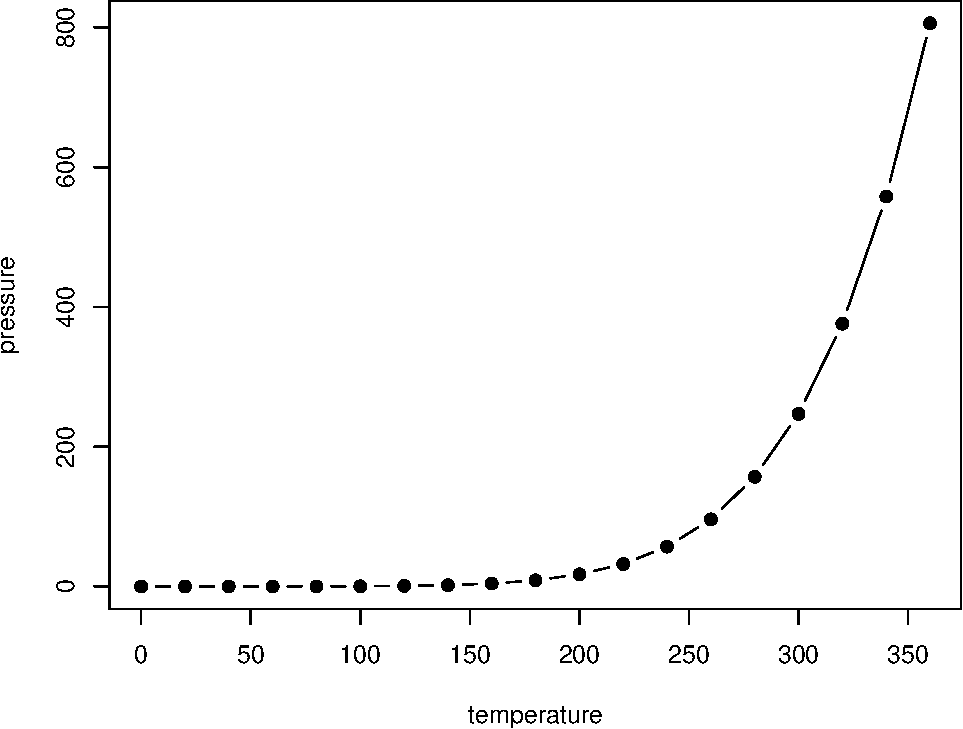
\includegraphics[width=0.8\linewidth,alt={Plot with connected points showing that vapor pressure of mercury increases exponentially as temperature increases.}]{_main_files/figure-latex/nice-fig-1} 

}

\caption{Here is a nice figure!}\label{fig:nice-fig}
\end{figure}

Don't miss Table \ref{tab:nice-tab}.

\begin{Shaded}
\begin{Highlighting}[]
\NormalTok{knitr}\SpecialCharTok{::}\FunctionTok{kable}\NormalTok{(}
  \FunctionTok{head}\NormalTok{(pressure, }\DecValTok{10}\NormalTok{), }\AttributeTok{caption =} \StringTok{\textquotesingle{}Here is a nice table!\textquotesingle{}}\NormalTok{,}
  \AttributeTok{booktabs =} \ConstantTok{TRUE}
\NormalTok{)}
\end{Highlighting}
\end{Shaded}

\begin{table}

\caption{\label{tab:nice-tab}Here is a nice table!}
\centering
\begin{tabular}[t]{rr}
\toprule
temperature & pressure\\
\midrule
0 & 0.0002\\
20 & 0.0012\\
40 & 0.0060\\
60 & 0.0300\\
80 & 0.0900\\
\addlinespace
100 & 0.2700\\
120 & 0.7500\\
140 & 1.8500\\
160 & 4.2000\\
180 & 8.8000\\
\bottomrule
\end{tabular}
\end{table}

\chapter{Brain Dump / FAQ}\label{help}

Congrats you got through most of CBW's Bookdown Documentation!

\section{Danger Zones}\label{danger-zones}

\begin{itemize}
\tightlist
\item
  renaming your file with this project, doesn't change the .Rprog file!
\end{itemize}

Ex. Forgot to pull before editing?
- Your git window will say (at the top of the window) your branch is ahead of the main branch
- You will probably have to deal with a merge conflict
- {[}this is pretty in-depth{]}

\section{Potential Errors \& Bugs}\label{potential-errors-bugs}

Trying to build and getting \textbf{``Exited with status 1.''}? Bad news: Your book is not building properly. Good news: here are some \emph{(hopefully)} helpful debugging tricks.

\begin{itemize}
\item
  **``Error: LaTeX failed to compile \_main.tex.''** - Essentially, something in your code is not allowing the output to be produced properly. Something in your code is producing incorrect output that is not allowing output to be produced.
  \textgreater{} TIP: Try to comment out recent changes. Try to decipher what exactly caused the build to fail. This will help you find your bug.
\item
  \textbf{{[}X{]}.html not found} - This may result in bad syntax that creates a faulty file. First, fix whatever bug caused that faulty file to occur. Then, rebuild. If you continue to get this error, it may be because the rebuild did not delete the previous faulty html file. Try deleting the docs file and rebuilding. (This can be a good debug solution in general!)
\item
  If you get a bug where your website builds into a website that looks like it is made using very simple html, you may have to change your permissions. If you see \textbf{``Permission denied''} in your warning messages, trying running this command \texttt{chmod\ -R\ u+w\ docs} in terminal, in the folder containing your docs folder {[}CLARIFY ?{]}
\item
  \textbf{``Could not produce X output''} - by default, bookdown builds all possible formats: gitbook, pdf, epub versions. We only need the gitbook, so if you're having issues, change your build settings to only creating the gitbook {[}CLARIFY + INCLUDE IMAGES{]}
\item
  A very common bug is \textbf{``missing X package''}, just install it using this command in your console (the bottom left window in RStudio) \texttt{install.packages("missing\ package\ name,\ include\ these\ surrouding\ quotations")}
\item
  Not being able to produce a specific format - If you're getting one of the following errors:

  \begin{itemize}
  \tightlist
  \item
    bookdown::render\_book() \textbf{failed to render the output format} `bookdown::pdf\_book'
  \item
    bookdown::render\_book() failed to render the output format `bookdown::epub\_book'
  \end{itemize}

  There is an easy fix! Press the dropdown options in the ``Build Book'' button and select ``bookdown::gitbook''. We only need to produce the gitbook (the html pages!) so it's ok if we can not produce the other pages. (However, it is ideal if we could produce all format types, since not being able to may lead to more errors.) This was likely due to creating something in one of the other formats that does not work in that format. For example:

\begin{verbatim}
  - **"File '..._svg-tex.pdf' is missing."** is a bug that only occurs when producing bookdown::pdf_book. It occurs since you are calling a svg image in regular markdown, which is not allowed. If you want to display a .svg image, use HTML code. 
\end{verbatim}
\end{itemize}

\section{Ease of Use}\label{ease-of-use}

\subsection{Wrapping Your Code}\label{wrapping-your-code}

Sometimes, RStudio defaults so that there is no text wrapping when viewing your files. If you notice that you have to scroll horizontally to see the long lines in your files, turn on ``Soft-Wrap Long Lines''.

\begin{enumerate}
\def\labelenumi{\arabic{enumi}.}
\item
  In your upper left corner of your RStudio Window, you will see options ``File'', ``Edit'', ``Code''. (If you are in full-screen on a mac, you will have to bring your cursor to the upper left corner before seeing these options). Click ``Code''.
\item
  Go to the 5th option ``Soft-Wrap Long Lines'' and select it.
\end{enumerate}

\subsection{Visual R Markdown}\label{visual-r-markdown}

If you are having difficulties using Markdown Syntax, RStudio has a work around! See \hyperref[visual-r-md]{Visaul R Markdown} for more information.

\section{FAQs}\label{faqs}

\begin{enumerate}
\def\labelenumi{\arabic{enumi}.}
\item
  I made a change via GitHub and and it's not appearing on the website. Why can I not see my edit?

  Let's recall this image.

  We build our \textbf{HTML} files using Bookdown. This means, any edits we make have to be local, so we can build our website and have the changes in our HTML files. GitHub Pages (which generates our website) only looks at the HTML pages, so even though there is a change on GitHub, it is on the .Rmd files. Hence, we don't see it on the actual website!

  Next Step: Git Pull your change locally. Build the website. Git Push and then see your edits once the website finishes deploying!
\end{enumerate}

\part{DEVELOPERS GUIDE}\label{part-developers-guide}

\chapter{Build Site}\label{build-site}

\section{How to edit \_bookdown.yml}\label{how-to-edit-_bookdown.yml}

\begin{itemize}
\tightlist
\item
  add a new line, \texttt{output\_dir:\ "docs"} to \_bookdown.yml
\item
  build the site
\item
  add a \texttt{.nojekyll} file into the produced docs folder
\end{itemize}

\section{How to edit \_output.yml (RC)}\label{how-to-edit-_output.yml-rc}

\begin{itemize}
\tightlist
\item
  after \emph{before:} change your workshop name link
\item
  after \emph{edit:} put the link to the workshop repo, and end the link with \texttt{/\%s}
\item
  save
\end{itemize}

\section{Mandatory ``index.Rmd'' landing page}\label{mandatory-index.rmd-landing-page}

Each \textbf{bookdown} chapter is an .Rmd file, and each .Rmd file can contain one (and only one) chapter. A chapter \emph{must} start with a first-level heading: \texttt{\#\ A\ good\ chapter}, and can contain one (and only one) first-level heading.

Use second-level and higher headings within chapters like: \texttt{\#\#\ A\ short\ section} or \texttt{\#\#\#\ An\ even\ shorter\ section}.

The \texttt{index.Rmd} file is required, and is also your first book chapter. It will be the homepage when you render the book.

\section{Build the book:}\label{build-the-book-1}

\begin{itemize}
\tightlist
\item
  ``Build'' button in RStudio IDE /OR/ bookdown::render\_book()
\item
  Preview the book: - updates on saves in viewer window bookdown::serve\_book()
\end{itemize}

Before building

\subsection{Render book}\label{render-book}

You can render the HTML version of this example book without changing anything:

\begin{enumerate}
\def\labelenumi{\arabic{enumi}.}
\item
  Find the \textbf{Build} pane in the RStudio IDE, and
\item
  Click on \textbf{Build Book}, then select your output format, or select ``All formats'' if you'd like to use multiple formats from the same book source files.
\end{enumerate}

Or build the book from the R console:

\begin{Shaded}
\begin{Highlighting}[]
\NormalTok{bookdown}\SpecialCharTok{::}\FunctionTok{render\_book}\NormalTok{()}
\end{Highlighting}
\end{Shaded}

To render this example to PDF as a \texttt{bookdown::pdf\_book}, you'll need to install XeLaTeX. You are recommended to install TinyTeX (which includes XeLaTeX): \url{https://yihui.org/tinytex/}.

\subsection{Preview book}\label{preview-book}

As you work, you may start a local server to live preview this HTML book. This preview will update as you edit the book when you save individual .Rmd files. You can start the server in a work session by using the RStudio add-in ``Preview book'', or from the R console:

\begin{Shaded}
\begin{Highlighting}[]
\NormalTok{bookdown}\SpecialCharTok{::}\FunctionTok{serve\_book}\NormalTok{()}
\end{Highlighting}
\end{Shaded}

\chapter{Git Instructions}\label{git-instructions}

\section{How to Make a Git Repo (RC)}\label{how-to-make-a-git-repo-rc}

\begin{enumerate}
\def\labelenumi{\arabic{enumi}.}
\item
  Go to \url{https://github.com/cbw-dev} (CHANGE?) and scroll to your repositories.
\item
  Click the green ``New'' button to the right of the repositories search bar.
\item
  Create the new repository. Give it a \emph{name} and \emph{description}. Select \emph{Public} instead of private, as shown below.
\end{enumerate}

\begin{quote}
🚧 Warning

MAKE NAMING CONVENTION
\end{quote}

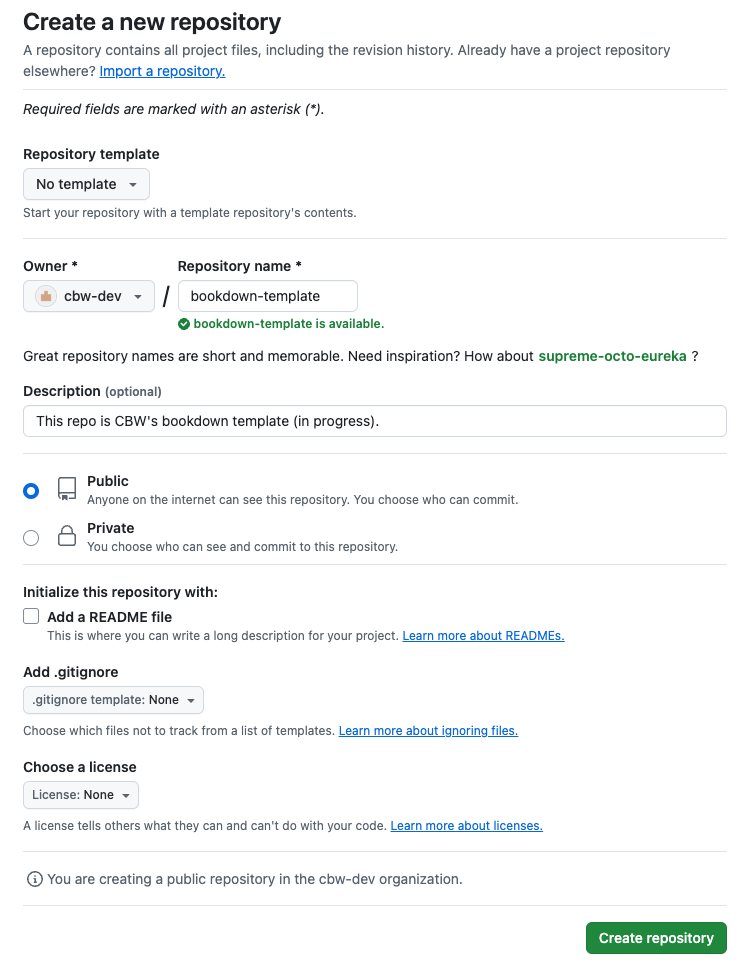
\includegraphics{img/git-instruct/create-git-repo.png}
4. Click the green \emph{Create repository} button at the bottom.

Now, we already have a local project. Now we want it on GitHub, so everyone on your team can make changes to the workshop! Let's make the GitHub connection (i.e let's add our local code to GitHub!)

\subsection{How to Make the Git Connection (Adding your Local Repo to GitHub)}\label{how-to-make-the-git-connection-adding-your-local-repo-to-github}

After the previous step, you will be brought to this page.The only things that will differ are the name of the repo.

\begin{figure}
\centering
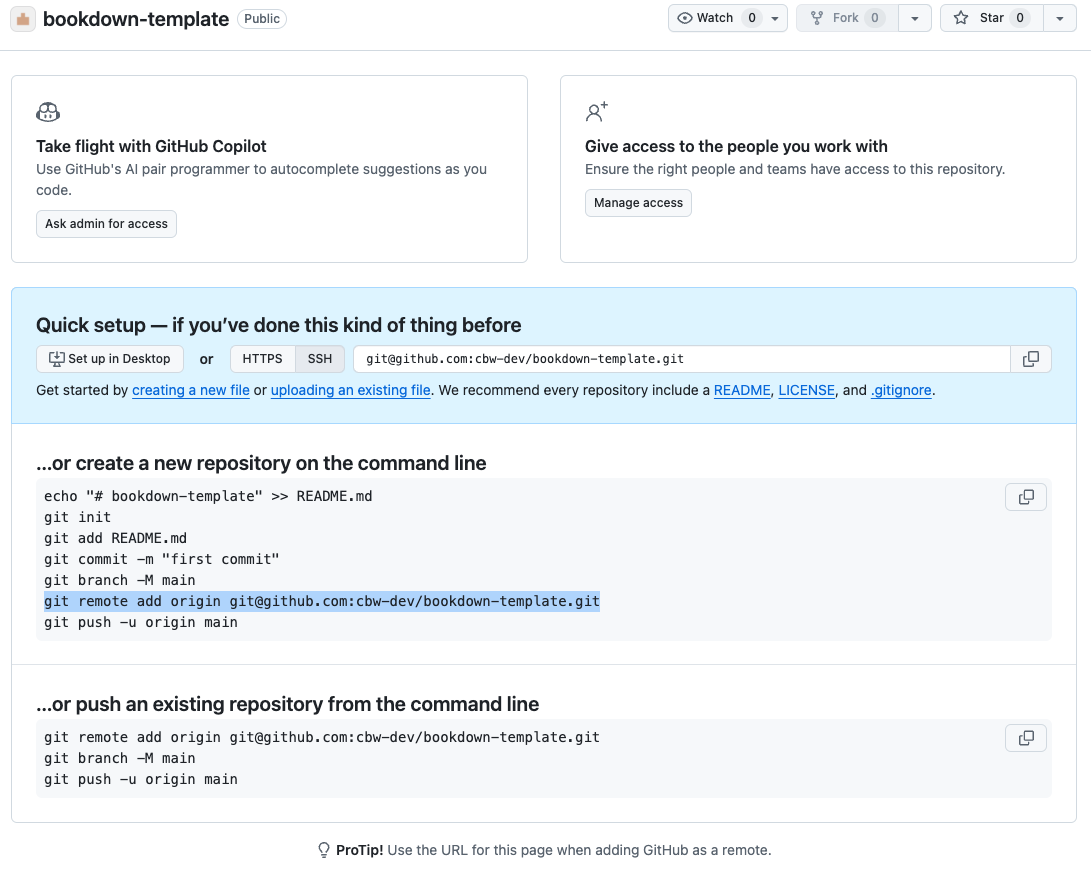
\includegraphics{img/git-instruct/git-connection.png}
\caption{landing page after making a git repo}
\end{figure}

\begin{enumerate}
\def\labelenumi{\arabic{enumi}.}
\setcounter{enumi}{4}
\item
  Open Terminal (Mac) or Command Prompt/Powershell (Windows).
\item
  Go to where we created the bookdown project.
\item
  Once inside the folder with the project. Let's make the git repo. First we initialize: \texttt{git\ init}. (Put this into terminal and press enter.)
\item
  Let's add all the files: \texttt{git\ add\ *}
\item
  Let's commit these files, with a descriptive message to help make it clear to others what we just did. For now, our message can be simple: \texttt{git\ commit\ -m\ "first\ commit"}. (Put this into terminal and press enter.)
\item
  Next, put this into terminal and press enter: \texttt{git\ branch\ -M\ main}.
\item
  \textbf{Important:} This step is why I highlighted that specific text above. Copy that command, and put it into terminal. Generally, it will look something like this: \texttt{git\ remote\ add\ origin\ git@github.com:cbw-dev/NAME-OF-YOUR-REPO.git}
\item
  Next, put \texttt{git\ push\ -u\ origin\ main} into terminal and press enter.
\end{enumerate}

All the steps are shown below.

\begin{figure}
\centering
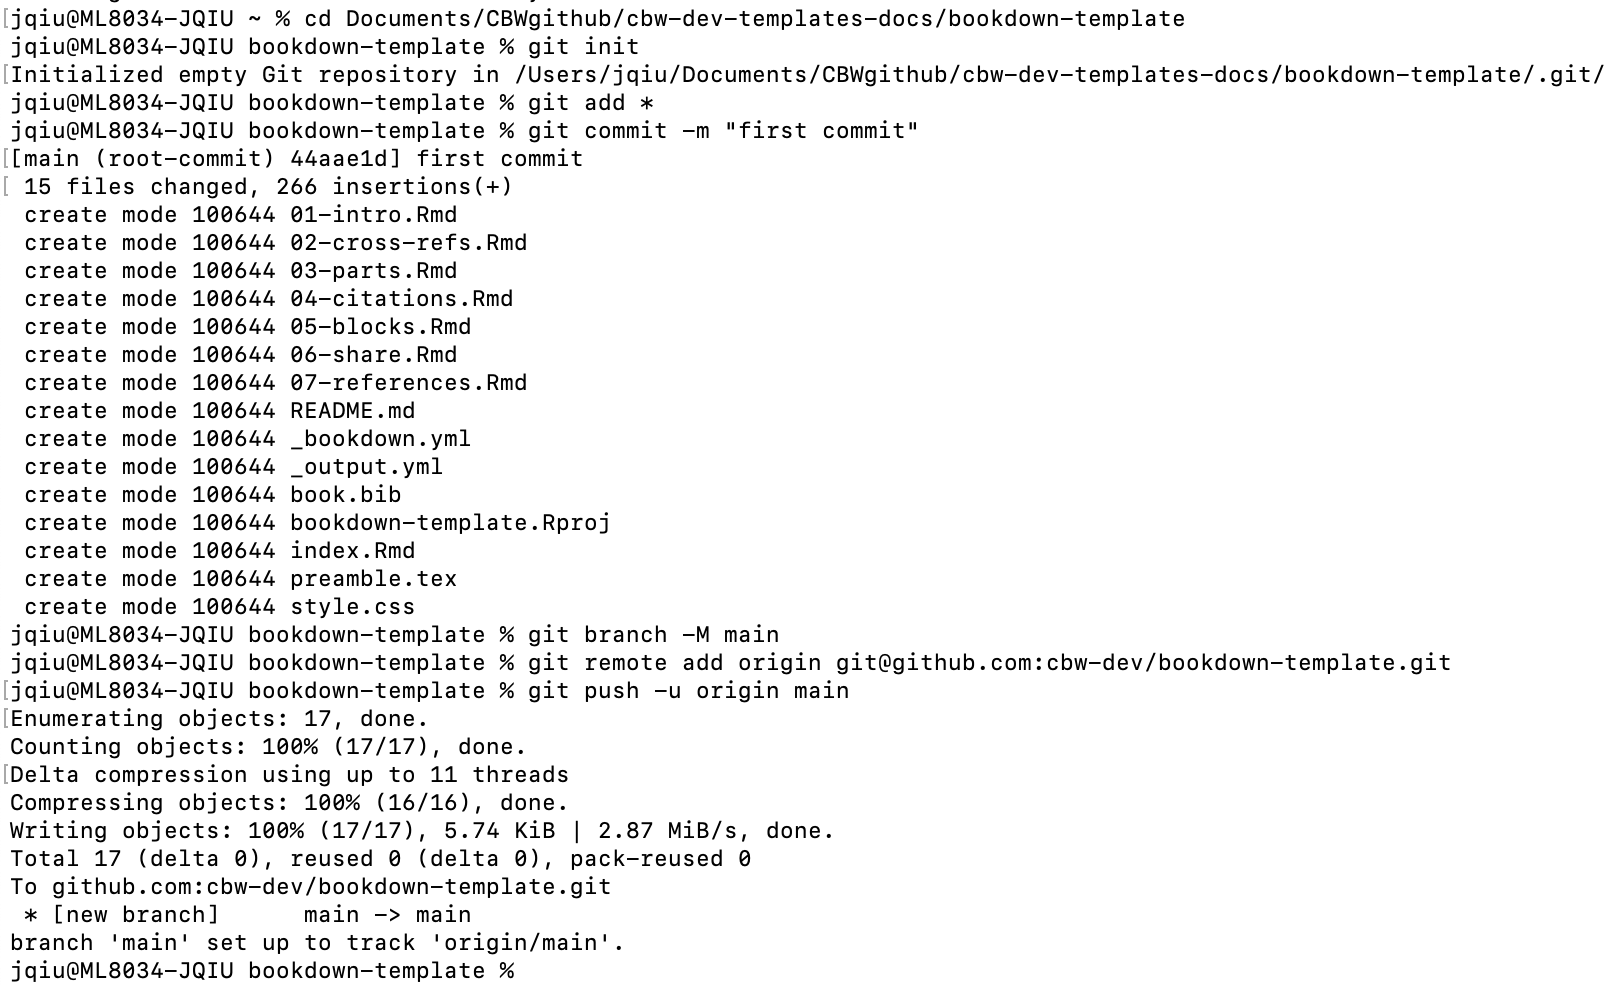
\includegraphics{img/git-instruct/git-instructions-in-terminal.png}
\caption{all the git steps typed out into terminal with results}
\end{figure}

\section{Updating GitHub via RStudio}\label{updating-github-via-rstudio}

Now, close your RStudio session, and reopen it.

Now, we will be able to see a Git window in the top right. Click ``Git'' to open this window.

\begin{figure}
\centering
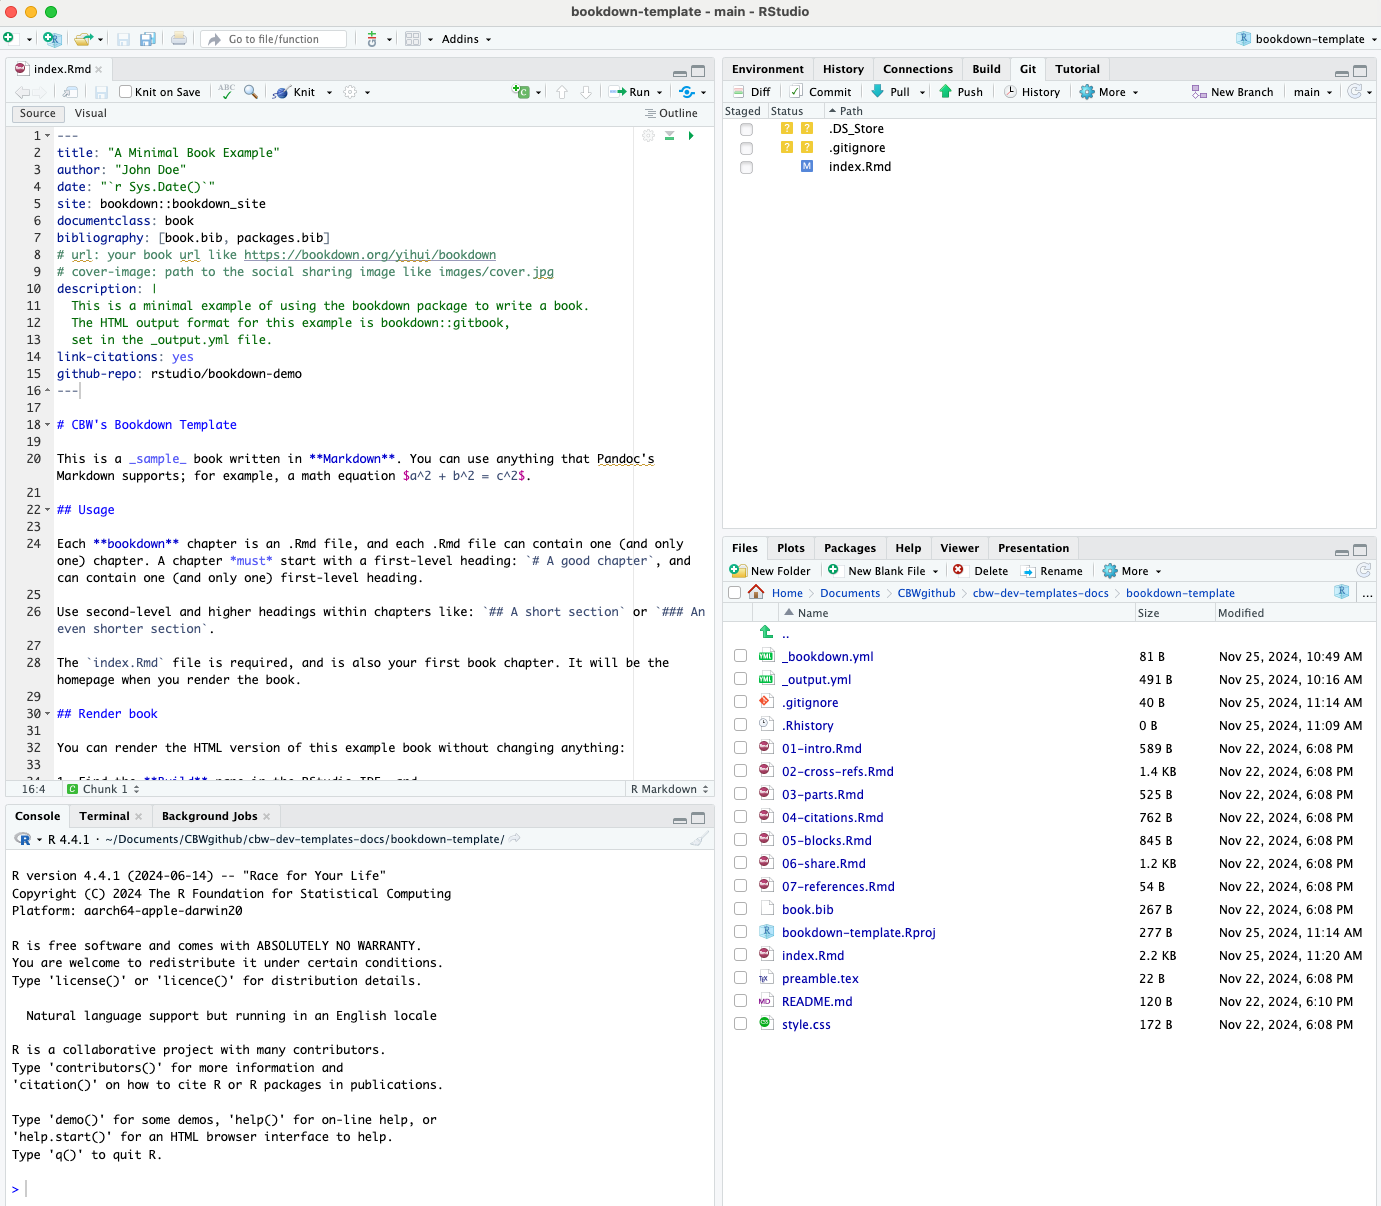
\includegraphics{img/git-instruct/RStudio-with-git-window-open.png}
\caption{RStudio with Git window open}
\end{figure}

Let's say we only edited \texttt{index.Rmd}, now we see the newly edited files. (Do not worry too much about \texttt{.DS\_Store} and \texttt{.gitignore} do.) Let's try to push this change to GitHub.

\begin{enumerate}
\def\labelenumi{\arabic{enumi}.}
\setcounter{enumi}{12}
\tightlist
\item
  Select all the edited files.
\end{enumerate}

\begin{figure}
\centering
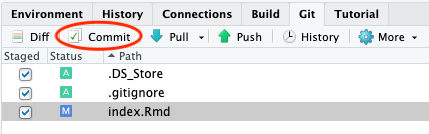
\includegraphics{img/git-instruct/git-window-selected-items.png}
\caption{selected files in the git window and the commit button highlighted}
\end{figure}

\begin{enumerate}
\def\labelenumi{\arabic{enumi}.}
\setcounter{enumi}{13}
\tightlist
\item
  Then, click the Commit button, which appears above your selected items. A window pane will appear (shown below).
\end{enumerate}

\begin{figure}
\centering
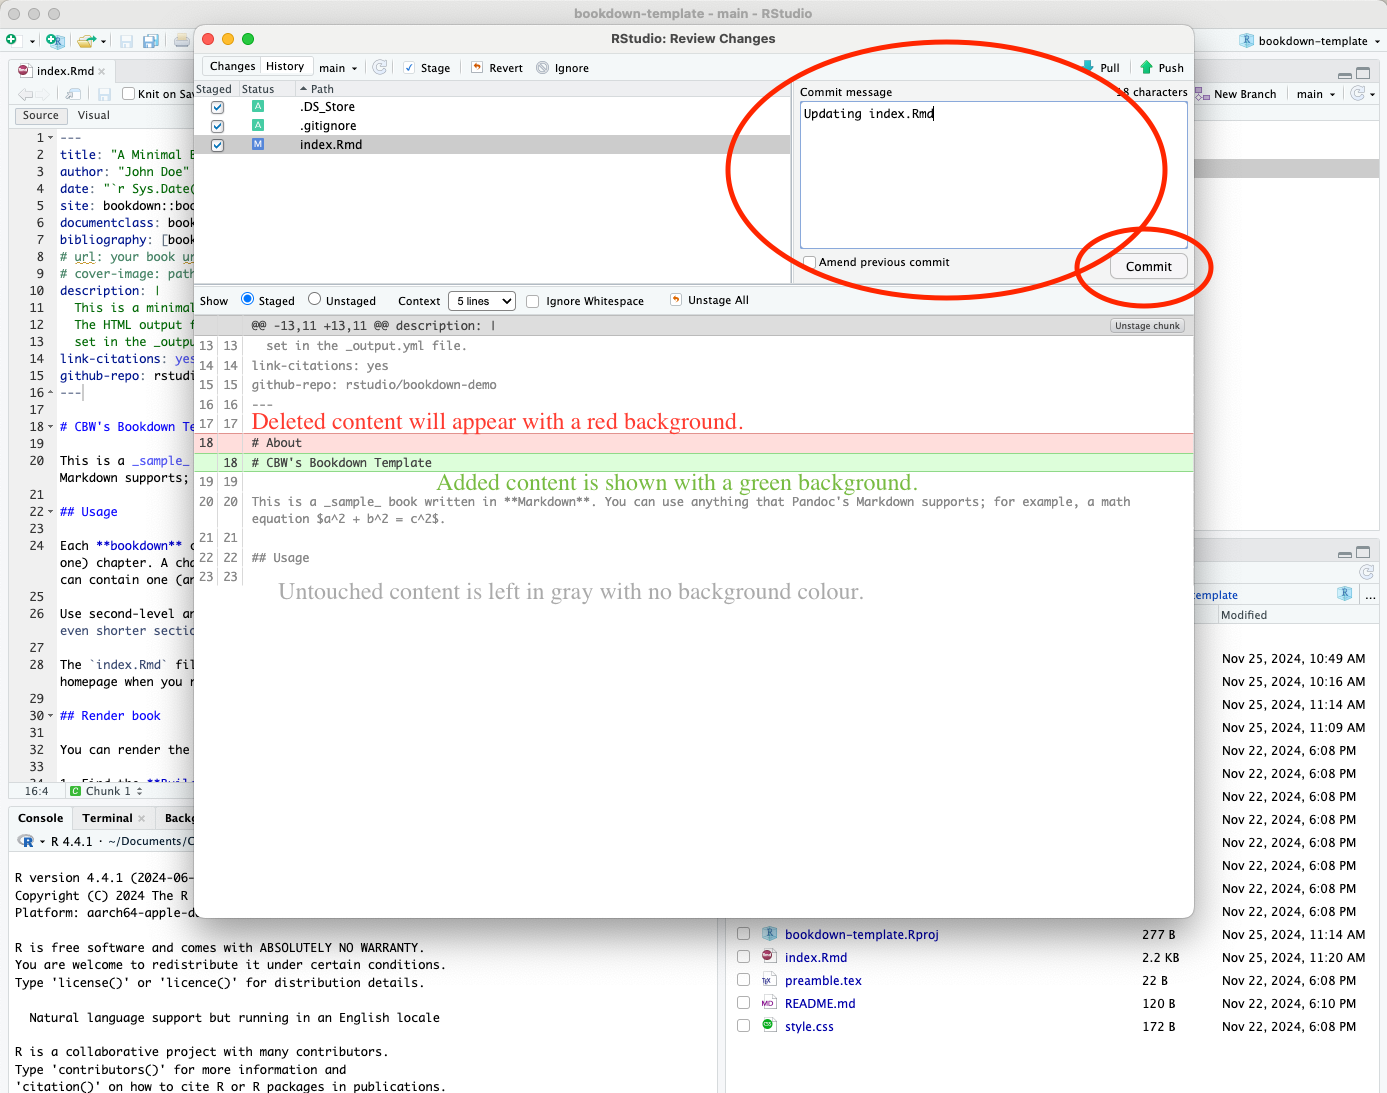
\includegraphics{img/git-instruct/git-commit-window.png}
\caption{git commit window pane}
\end{figure}

\begin{enumerate}
\def\labelenumi{\arabic{enumi}.}
\setcounter{enumi}{14}
\item
  Add a commit message in the corresponding box, and then press commit below it.
\item
  A new window will show up, detailing your updates. Close this window and then press \textbf{Push} to push your updates to GitHub.
\end{enumerate}

\begin{figure}
\centering
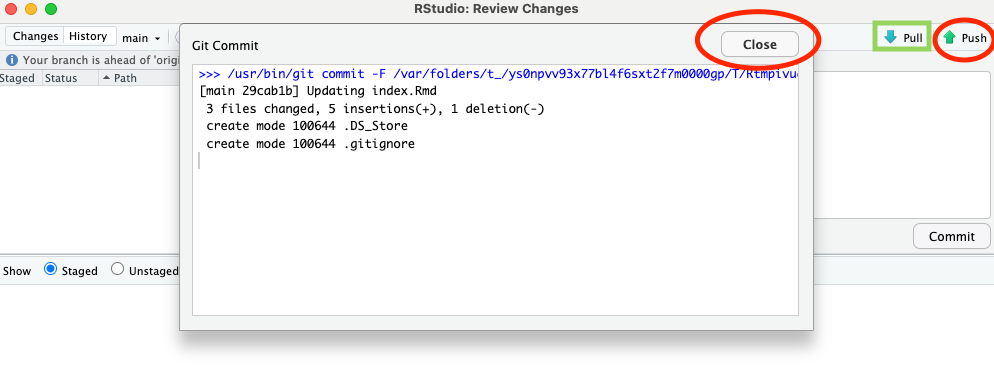
\includegraphics{img/git-instruct/git-window-post-commit.png}
\caption{post git commit window}
\end{figure}

Now, we're done! We should see the updates on GitHub now. Also note, if we ever want to pull updates from GitHub, there is also a \textbf{Pull} button in the Git window within RStudio!

\chapter{How to Deploy Your Workshop Website}\label{how-to-deploy-your-workshop-website}

Let's recap.

We've made a bookdown project that builds into a website. We've reconfigured the output to go to a folder called ``docs'' (output\_dir: ``docs''). We've pushed our content onto github, and also made a ``.nojekyll'' file, which we placed into docs.

Now in our ./docs folder, we have a bunch of html files that make up our website. We want GitHub to look at these files in the docs folder and host the website for us!

We deploy our website using GitHub pages. GitHub pages uses jekyll, so the .nojekyll file tells it to no longer rely on jekyll. Now, all we need to do is tell GitHub pages to deploy (create/update the website) from our docs folder.

\begin{enumerate}
\def\labelenumi{\arabic{enumi}.}
\item
  Go to your repo on GitHub.
\item
  In the top navigation bar, select settings.
  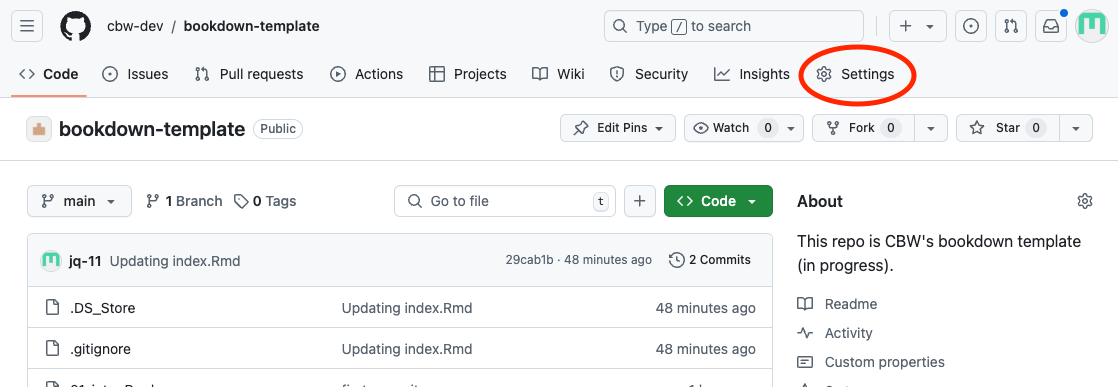
\includegraphics{img/git-instruct/github-settings.png}
\item
  Then, go to the pages sidebar.
  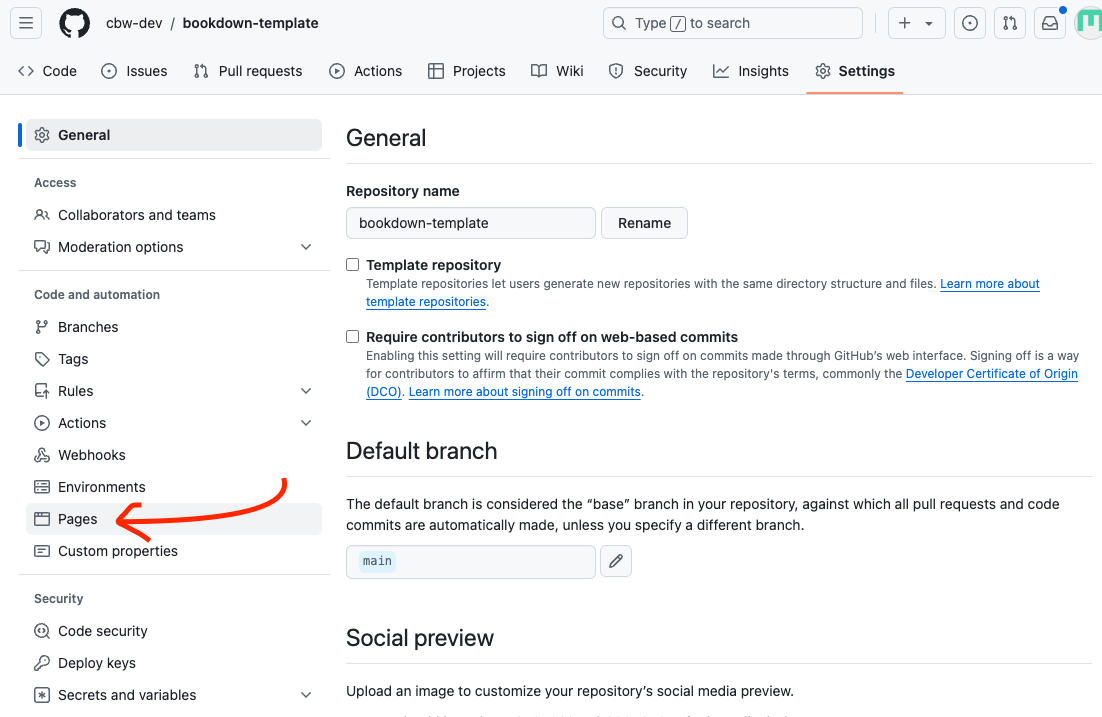
\includegraphics{img/git-instruct/github-select-pages.png}
\item
  ``Deploy from a branch'' is already selected, which is what we want. We must change the branch from ``none'' to main.
  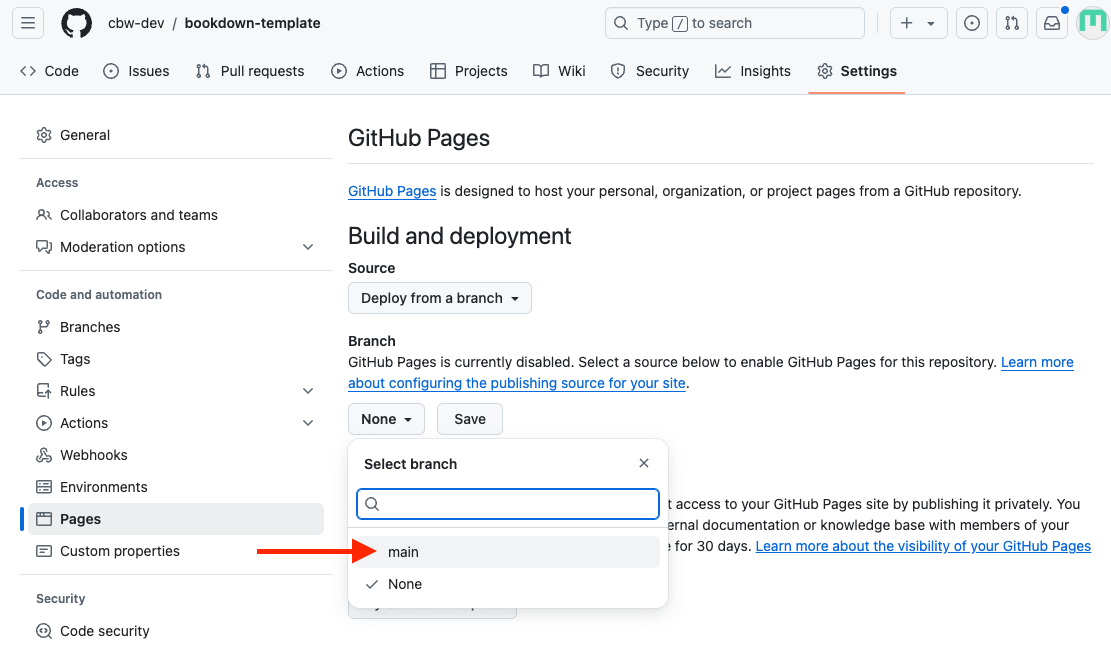
\includegraphics{img/git-instruct/github-deploy-main.png}
\item
  Then, change the folder from \texttt{/\ root} to \texttt{/docs}. Then press save.
  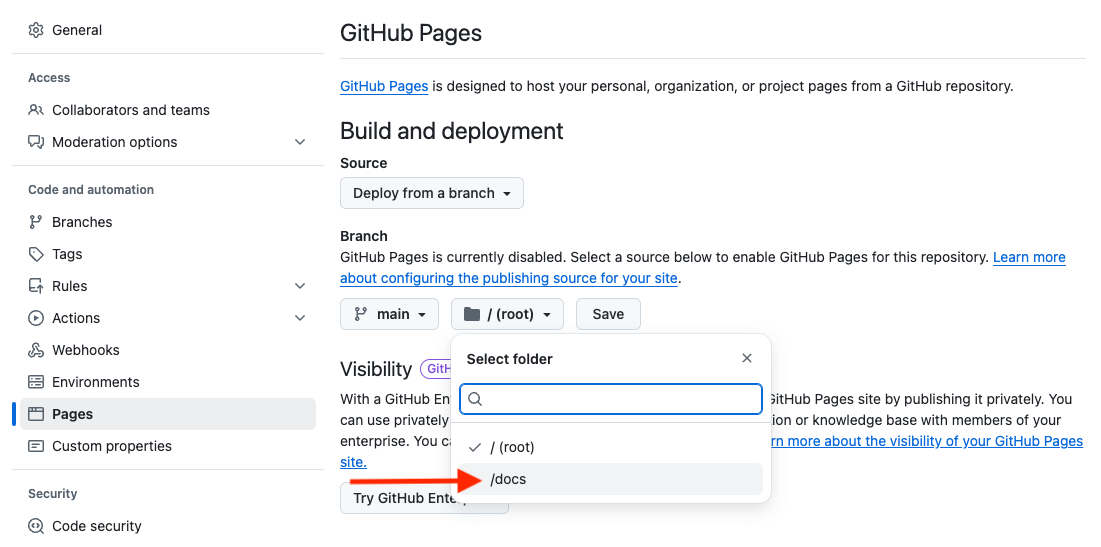
\includegraphics{img/git-instruct/github-deploy-docs.png}
\end{enumerate}

Great! Now we're waiting on the page to build and deploy, which should take less than a minute.

To see updates, go to the \textbf{Actions} page (found along the top navigation bar. This will help you understand how the deploy is working, and if it succeeded or failed.

\begin{figure}
\centering
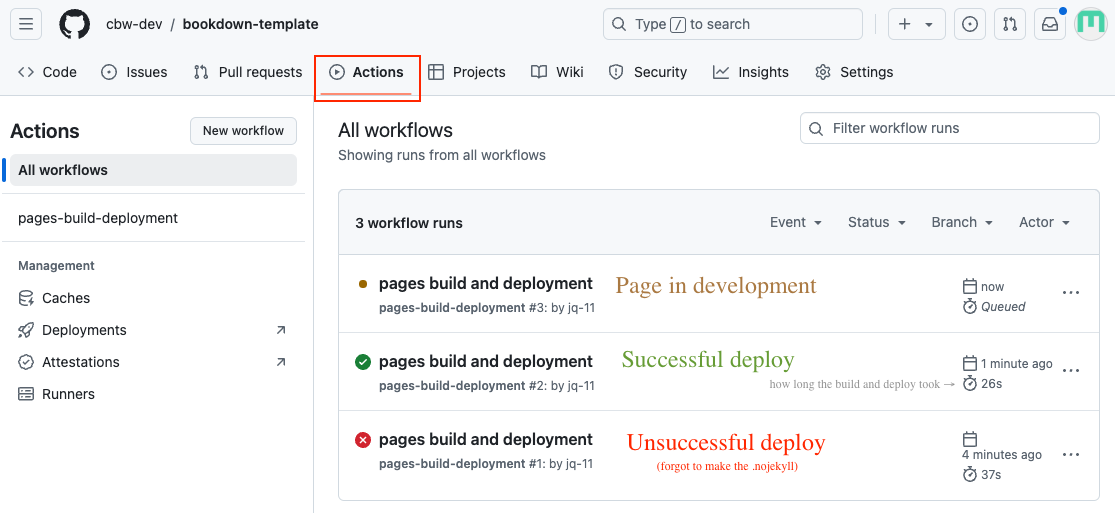
\includegraphics{img/git-instruct/github-pages-actions-explained.png}
\caption{Image showing the different possibilities of deploy a github page}
\end{figure}

You can click \textbf{pages build and deployment} for updates. It will give you errors (which may not be very clear) or the link of your deployed page!

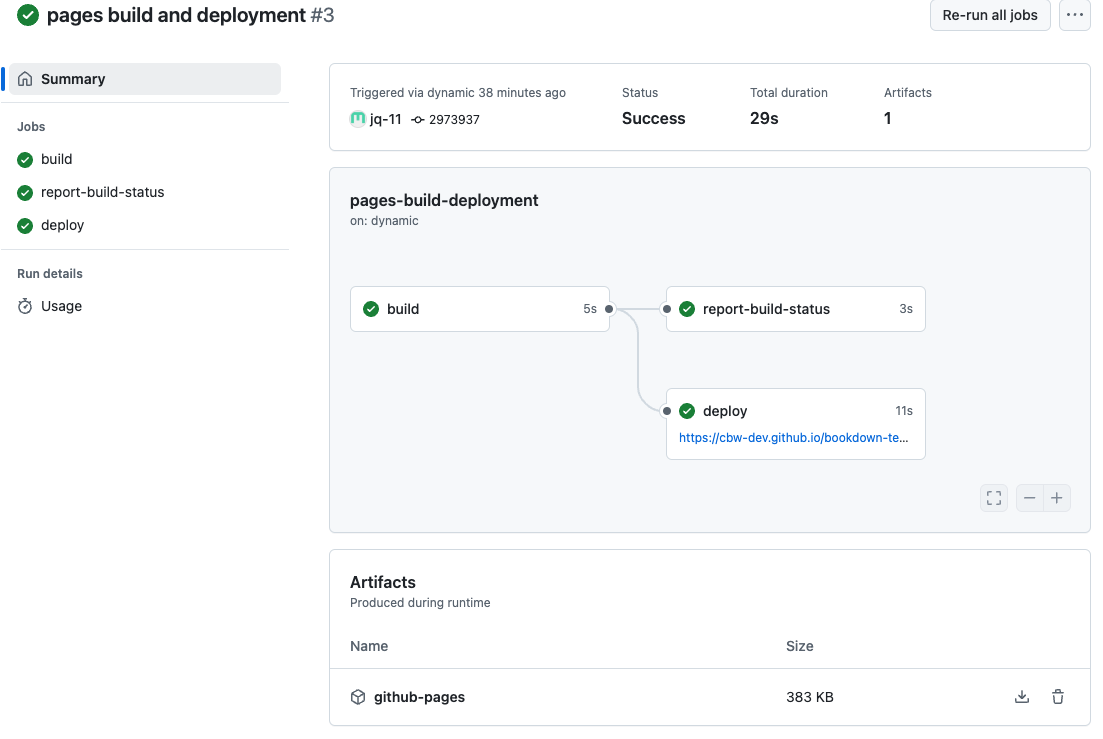
\includegraphics{img/git-instruct/successful-deploy.png}
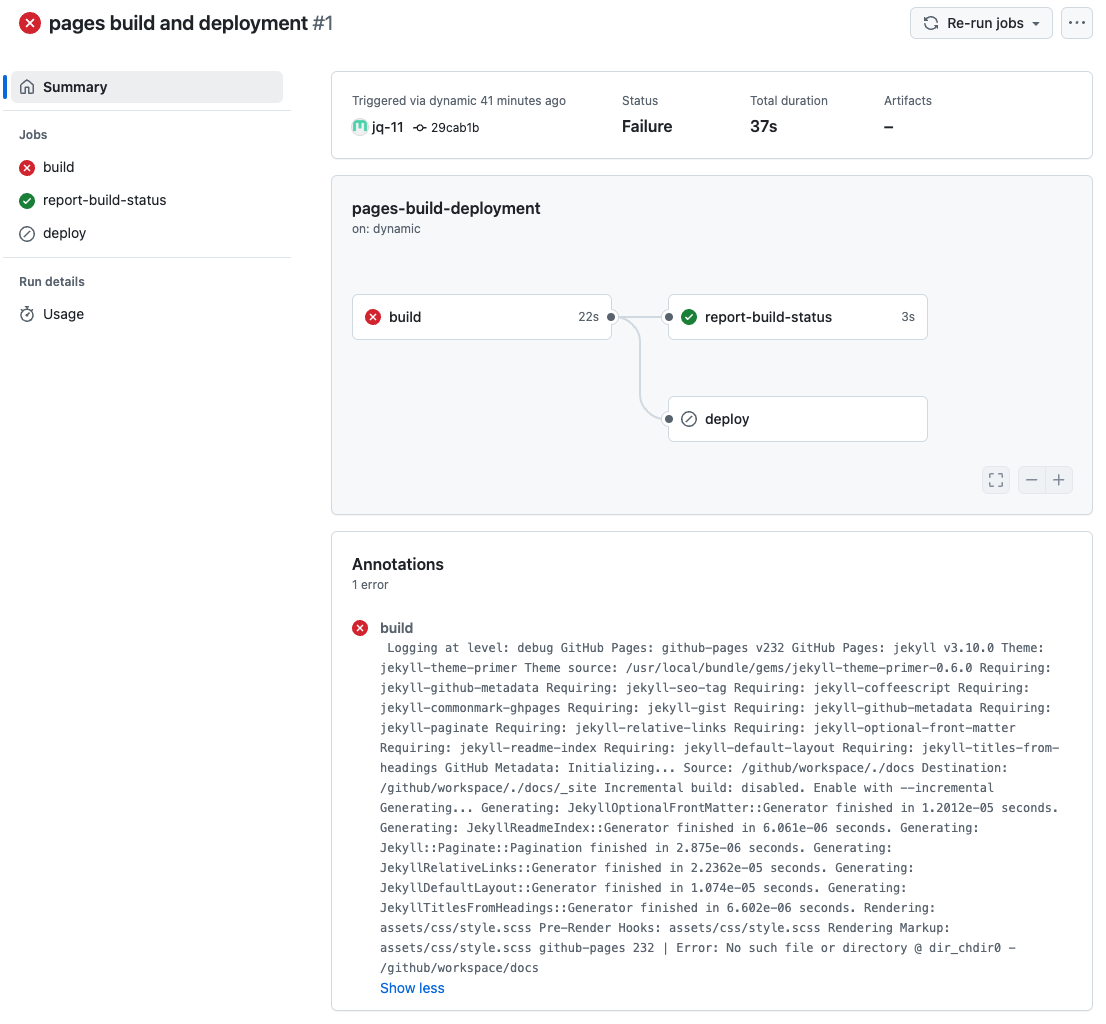
\includegraphics{img/git-instruct/failed-deploy.png}

Click around to explore more!

\chapter{Appendix {[}Links for Developers{]}}\label{appendix-links-for-developers}

For the developers of this guide, here are helpful sources.

\section{GitHub Repo}\label{github-repo}

The Bookdown Docs are hosted from the \href{https://github.com/cbw-dev/bookdown-docs}{cbw-dev/bookdown-docs} public repository.

\section{Diagram Links}\label{diagram-links}

Most diagrams shown on these docs \textbf{should} be in this \href{https://drive.google.com/drive/folders/136sy6WIiSG3tBFVpHt8yQwLakB4TFJvn?usp=sharing}{Google folder}.

\subsection{How to Edit a Google Drawing}\label{how-to-edit-a-google-drawing}

\begin{enumerate}
\def\labelenumi{\arabic{enumi}.}
\item
  Open the drawing.
\item
  Edit.

  \begin{quote}
  Tip: Editing size of the Google Drawing is very easy when you drag the diagonal lines in the bottom right corner.
  \end{quote}
\item
  To publish, go to ``File \textgreater{} Share \textgreater{} Publish to Web \textgreater{} Embed''. Copy the ``Medium'' \emph{(optional)} image size HTML code. Paste where you want it to appear in your .Rmd file.
\item
  Add alt text to the img embed code: Add \texttt{alt="Alt\ Text"} after \texttt{src\ =\ ...} and before \texttt{\textgreater{}}.
\end{enumerate}

Note: Lots of the GitHub clone/deploy/RStudio explaining images are currently locally in the repository, and not on the Google drive.

\textbf{References} (the below citation list is auto-generated since we showed examples of citations)

  \bibliography{book.bib,packages.bib}

\end{document}
